\documentclass[a4paper,oneside,12pt]{book}

\newcommand{\thesistitle}{French News Sentiment Analysis on COVID-19} % Your thesis title, this is used in the title and abstract
\newcommand{\degree}{B. A. (Mod.) Computer Science} % Your degree name, this is used in the title page and abstract
\newcommand{\typeofthesis}{dissertation} % dissertation, Final Year Project, report, etc.
\newcommand{\authorname}{Samuel Petit}

\newcommand{\keywords}{this, that, more} % Keywords for your thesis
\newcommand{\school}{\href{http://www.scss.tcd.ie}{School of Computer Science and Statistics}} % Your school's name and URL, this is used in the title page
\newcommand{\schoolAddress}{O’Reilly Institute, Trinity College, Dublin 2, Ireland} % Your school's name and URL, this is used in the title page

%% Comment out the next line if you don't want a department to appear
\newcommand{\trinity}{\href{https://www.tcd.ie/}{Trinity College}} 
\newcommand{\TRINITY}{\href{https://www.tcd.ie/}{TRINITY COLLEGE}} 

\AtBeginDocument{
\hypersetup{pdftitle=\thesistitle} % Set the PDF's title to your title
\hypersetup{pdfauthor=\authorname} % Set the PDF's author to your name
\hypersetup{pdfkeywords=\keywords} % Set the PDF's keywords to your keywords
\hypersetup{pdfsubject=\degree} % Set the PDF's keywords to your keywords
}

%% Language and font encodings
\usepackage[T1]{fontenc} 
\usepackage[utf8]{inputenc}
\usepackage[english]{babel}
\usepackage{csvsimple}

%% Bibliographical stuff
\usepackage[round,sort,comma,numbers]{natbib}

%% Document size
% include showframe as an option if you want to see the boxes
\usepackage[a4paper,top=2.54cm,bottom=2.54cm,left=2.54cm,right=2.54cm,headheight=16pt]{geometry}
\setlength{\marginparwidth}{2cm}
%% Useful packages
\usepackage{amsmath}
\usepackage[autostyle=true]{csquotes} % Required to generate language-dependent quotes in the bibliography
\usepackage[pdftex]{graphicx}
\usepackage[colorinlistoftodos]{todonotes}
\usepackage[colorlinks=true, allcolors=black]{hyperref}
\usepackage{caption} % if no caption, no colon
\usepackage{sfmath} %use sans-serif in the maths sections too
\usepackage[parfill]{parskip}    % Begin paragraphs with an empty line rather than an indent
\usepackage{setspace} % to permit one-and-a-half or double spacing
\usepackage{enumerate} % fancy enumerations like (i) (ii) or (a) (b) and suchlike
\usepackage{booktabs} % To thicken table lines
\usepackage{fancyhdr}

\pagestyle{plain} % Embrace simplicity!

\renewcommand{\familydefault}{\sfdefault} %use the sans-serif font as default

\renewcommand{\theequation}{\arabic{equation}} %% use continuous equation numbers

% Setup auto CSV to table commands 
\makeatletter
\csvset{
  autotabularcenter/.style={
    file=#1,
    after head=\csv@pretable\begin{tabular}{|*{\csv@columncount}{c|}}\csv@tablehead,
    table head=\hline\csvlinetotablerow\\\hline,
    late after line=\\,
    table foot=\\\hline,
    late after last line=\csv@tablefoot\end{tabular}\csv@posttable,
    command=\csvlinetotablerow},
  autobooktabularcenter/.style={
    file=#1,
    after head=\csv@pretable\begin{tabular}{*{\csv@columncount}{c}}\csv@tablehead,
    table head=\toprule\csvlinetotablerow\\\midrule,
    late after line=\\,
    table foot=\\\bottomrule,
    late after last line=\csv@tablefoot\end{tabular}\csv@posttable,
    command=\csvlinetotablerow},
}
\makeatother
\newcommand{\csvautotabularcenter}[2][]{\csvloop{autotabularcenter={#2},#1}}
\newcommand{\csvautobooktabularcenter}[2][]{\csvloop{autobooktabularcenter={#2},#1}}

%% Format Chapter headings appropriately
\usepackage{titlesec}
\titleformat{\chapter}[hang] 
{\normalfont\huge\bfseries}{\thechapter}{1cm}{} 

\title{\thesistitle}
\author{\authorname}

\frontmatter
\begin{document}
\begin{titlepage}

\center % Center everything on the page

%\Large University of Dublin\\[1.5cm] % Minor heading such as course title


\includegraphics[scale=0.35]{title/tcd.png}\\[2cm] 

%\large \trinity\\[1.5cm]

%----------------------------------------------------------------------------------------
%	TITLE SECTION
%----------------------------------------------------------------------------------------
\makeatletter
{ \huge \bfseries \thesistitle}\\[1.5cm] % Title of your document
 
\Large\authorname\\
{\large \today}\\[1cm] % Date, change the \today to a set date if you want to be precise

 
%----------------------------------------------------------------------------------------
%	TYPE OF THESIS SECTION
%----------------------------------------------------------------------------------------
\degree\\
Final Year Project  April 2021\\
Supervisor: Prof. Khurshid Ahmad\\[2cm]

\vfill

\Large \school\\[0.5cm]
\Large \schoolAddress

\vfill % Fill the rest of the page with whitespace

\end{titlepage}
\pagenumbering{roman}
\section*{\Huge{Declaration}}
\vspace{1cm}
I hereby declare that this \typeofthesis\ is entirely my own work and that it has not been submitted as an exercise for a degree at this or any other university.

\vspace{1cm}
I have read and I understand the plagiarism provisions in the General Regulations of the University Calendar for the current year, found at \url{http://www.tcd.ie/calendar}.
\vspace{1cm}

I have also completed the Online Tutorial on avoiding plagiarism `Ready Steady Write', located at \url{http://tcd-ie.libguides.com/plagiarism/ready-steady-write}.
\vspace{3cm}

Signed:~\rule{5cm}{0.3pt}\hfill Date:~\rule{5cm}{0.3pt}

\chapter*{Abstract}

TODO % no more that around 400 words on a separate page

\newpage
\onehalfspacing\raggedright %\raggedright turns off justification and hypenation

\section*{\Huge{Acknowledgements}}

TODO
% I would like to thank my supervisor Professor Khurshid Ahmad for introducing me to this topic and guiding me throughout this project. I started working on this topic with very little knowledge on the topics covered in this thesis and I have no doubt that your supervision and continued support throughout the year was a key factor in completing this project.

\tableofcontents

\mainmatter
\listoffigures
\listoftables
\chapter{Introduction}\label{Introduction}

This chapter will begin with an introduction to the motivation which led to this research project. It will be followed by a section proposing the research question then by the objectives that have been set to best address this question. Finally, this chapter will conclude with a structure to the remainder of the thesis.

\section{Motivation}\label{Motivation}
Looking back in history, it is clear that the world went and will go through many phases
whether it be a pandemic, a war or a revolution to name a few. What makes the recent COVID-19 pandemic particularly interesting is that it is the first to be spread throughout the world during the digital age, creating new behaviours on the web.   
In the context of a global pandemic in a digital age, the role of news agencies is more important than ever, with the world population in quarantine all looking for the same information, seeking to understand the situation they are in.

One could manually read newspaper articles from many different sources about a topic in an attempt to understand how information is conveyed to the population, however such a study would be limited in the manpower available and would require a strict, well defined approach to do so. Taking such an approach is thus limited in its nature.

Natural Language Processing (NLP) is a sub-field of computer science which enables analysis of text, Sentiment Analysis makes use of NLP in order to extract subjective information from texts. Examples of this include extracting and quantifying the polarity or certain emotions from text.
To this day, most of the studies performed and the applications of Sentiment Analysis have been focused on the English language, leaving space for many new studies, specifically in languages that are constructed significantly differently such as French.

The French media publishes vast amounts of news articles daily, all of which can be used to extract meaningful information such as to ultimately understand hidden patterns in how information is communicated to the population in the context of a global emergency that is the COVID-19 pandemic.
This thesis attempts to automate the process of discovering such hidden patterns through the use of sentiment analysis on french news.

\section{Research Question}\label{Research Question}

The research question for this thesis can be summarized as follows:

\begin{center}
    \emph{To what extent does the sentiment of French news media relate to France's pandemic metrics?}
\end{center}

\section{Research Objectives}\label{Research Objectives}
To structure the work done and address the research question effectively, the following key objectives were defined:
\begin{enumerate}
    \item Gather a large corpus containing high quality french news articles relevant to COVID-19
    \item Create specialised dictionaries targeted to measure pandemic-related sentiments
    \item Perform sentiment analysis on the corpus to retrieve measures for various sentiments and term frequencies
    \item Conduct statistical analysis on the results in order to identify and quantify potential relationships
\end{enumerate}

\section{Report Structure}\label{Report Structure}

The next chapter will start with a look into the current literature on the role of the media in the context of a global emergency such as the COVID-19 pandemic (Chapter \ref{Literature Review}). This is followed by a review and discussion of the current literature for sentiment analysis, which will cover the main approaches used for its various applications. This chapter concludes with a discourse of the statistical methods used throughout this report.

The literature review is followed by a section on the method used (Chapter \ref{Method}). The method includes details of the approach taken to solve the research objectives previously laid out. It is split into three parts: data gathering which focuses on constructing and collecting data for the analysis, sentiment analysis which details the actions performed on the corpus to measure various sentiments and finally a section on the statistical analysis performed.

The following section (Chapter \ref{Evalutation}) discusses the results obtained from applying the method as previously described. It will begin with a review of the built corpus and include some initial analysis. Following will be the results of the corpus through the use of sentiment analysis and various dictionaries, some of which were built specifically for this study. This chapter will close with a discussion of the statistical analysis performed on the obtained metrics.

Finally, this report concludes with a review of the method which was used to perform this study (Chapter \ref{Conclusion}). Then a commentary on the key findings and the possible improvements will be carried out which outlines directions for future work. The thesis will come to an end with final comments on the project, providing insights into the challenges that were encountered and a brief reflection on the personal achievements that were made throughout this project.

\chapter{Literature Review}\label{Literature Review}

\section{The Media}

\subsection{Role of the Media in a crisis}\label{Role of the Media in a crisis}

TODO

\subsection{French Press}\label{chap:French Press}

TODO: possibly include some history of french press, AFP and more
% Find what the role of the press is, should be specifically in the context of important, hurtful events
%How the people see the covid 19 pandemic

\section{Sentiment Analysis}\label{Sentiment Analysis}

Sentiment Analysis (or opinion mining), is "the task of finding the opinions of authors about specific entities" \citep{feldman2013techniques}. It is a sub-field of Natural Language Processing (NLP) which has been growing in interest on a worldwide scale for over 15 years thanks to its vast range of use cases (Figure \ref{fig:sentiment interest}).

\begin{figure}[h!]
      \centering
      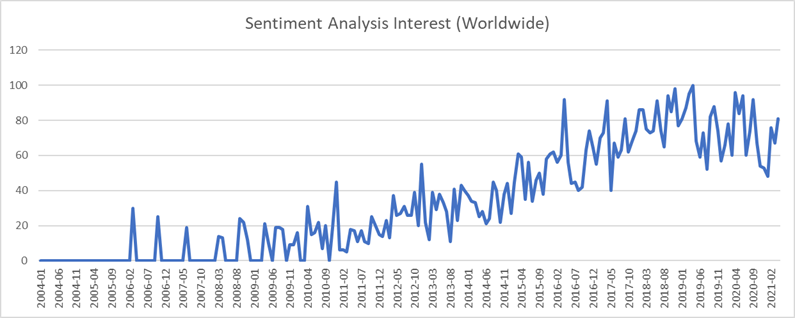
\includegraphics[scale=0.65]{lit_review/sentiment_analysis_interest.png}
      \caption{Sentiment Analysis Interest}
      \label{fig:sentiment interest}
      \emph{Source: Google Trends}
\end{figure}

In fact, sentiment analysis has been used in a wide range of topics, including political analyses of social and news media \citep{ahmad2011new}, stock market behaviors \citep{rao2012analyzing,li2014news}, customer sentiment \citep{cambria2013new,mouthami2013sentiment}, fake news detection \citep{bhutani2019fake} and countless more applications.

Languages are full of ambiguity and in particular the french language as some words can have drastically different meanings even though they are written the same, or adding an accent from a large variety of options can drastically change a words meaning. On top of this, it was found that a select set of words make up the majority of text, in fact, using a frequency-rank, it was found that the first 100 words make up for about 50\% of all of the words in a text cluster \citep{ahmad2007being}, this observation means that the interpretation of these highly frequent words is key to extracting sentiment proxies from text. While short text such as tweets \citep{chandrasekaran2020topics} or customer reviews can include a single sentiment or topic. It is not always the case and as the length of text grows more and more conflicting opinions are likely found. A simple example of this can be found on a customer review for a product: "I liked using the product, however I wish it didn't break after a day" where clearly both a positive and negative sentiment can be extracted from this review. This shows that there are multiple ways to perform sentiment analysis on text. Document-level computes the overall sentiment of a piece of text such as a tweet or a review, on the other hand, a sentence-level analysis approach can also be taken where a distinction is made between factual sentences (objective phrases) and subjective sentences which mostly contain opinions (subjective phrases) \citep{wilson2009recognizing}. A sentence-level approach is often used for tasks such as text summarizing, on the other hand, a document-level approach is often used for reviews or social media posts. 

Thankfully, some NLP techniques have now been standardised to help with these issues. One of the most important ones being the use of stemming or lemmatising. Both of these techniques transform words into a more basic version of that word, 

TODO: detail sections on lexicon / ml, lemmatization vs stemming and more (note: may be worth mentioning regexp)

\subsection{TODO}

TODO: lemmatization stemming, ml / lexicons. SpaCy \& treetagger lemmatizer. Etc
%\subsection{Lemmatization}
\label{lemmatization}

%compare treetagger and SpaCy -- show mean scores.
% look into ML vs Lexicon, stemming vs lemmas
% look into language issue English vs others
% french dictionaries

\section{French Lexica}\label{French Lexicons}

\subsection{FEEL}\label{chap: feel}

TODO

\subsection{Diko}\label{chap: diko}

TODO

\subsection{Polarimots}\label{chap: polarimots}

TODO

\section{Statistical Methods}\label{Statistical Methods}

The use of various statistical methods represent a key element for this thesis, as specified in the research objectives (Chapter \ref{chap: Research Objectives}). Such methods provide the link between observed values and identifying potential relationships. The various statistical methods used throughout this thesis will be introduced in the following sections.

\subsection{Core Statistics}

This first section introduces key, core statistic measures which are used throughout this thesis.

\subsubsection{Mean}

The mean is a very well known statistical measure which consists of the sum of the deviation of all of the values in a sample by the size of that sample. In other words, it is the average value in a sample. It is commonly referred to as $\bar{x}$ for a sample as well as $\mu$ for a population. It can be written as such:

\begin{equation}
    \mu = \bar{x} = \frac{1}{N}\sum^{N}_{i=1} x_{i}
\end{equation}
Where N is the sample size and $x_{i}$ represents the ith value in the sample.

\subsubsection{Variance and Standard Deviation}

The standard deviation and variance are related. A common symbol for the standard deviation is $\sigma$ for a population and $S$ for a sample. Given the standard deviation $S$ or $\sigma$ then the variance is its squared value: $S^{2}$ or $\sigma^{2}$.

The standard deviation measures how much data diverges from the mean. A low value indicates that the data is clustered around the mean, on the other hand a high standard deviation indicates that the sample is more spread out. The variance also measures how distributed data is relative to the mean in the same manner, except in much larger values as it is squared.

The mathematical formulas for computing the standard deviation and variance for a sample are the following:
\begin{equation}
    S = \sqrt{\frac{\sum_{i=1}^{N}(x_{i} - \bar{x})^{2}}{N - 1}}
\end{equation}
\begin{equation}
    S^2 = \frac{\sum_{i=1}^{N}(x_{i} - \bar{x})^{2}}{N - 1}
\end{equation}

\subsubsection{Skewness}

Similar to the variance and standard deviation, the skewness also measures data distribution. The skewness measures the degree of asymmetry from a normal distribution, in other words, it quantifies the difference between a sample distribution and the normal distribution.

Hence, the skewness for a normal distribution is 0. A positive skewness indicates that the data is skewed to the right, in other words the right tail is longer than the left. On the other hand, a negative skewness indicates that the data is skewed to the left. Figure \ref{skewness fig} illustrates this concept. Mathematically, it is written as such:

\begin{equation}
    skewness = \frac{\sum_{i=1}^{N}(x_{i} - \bar{x})^{3}}{(N - 1) * S^{3}}
\end{equation}
Where N is the sample size, $x_{i}$ is the ith data point from the sample, $\bar{x}$ is the mean and $S$ is the standard deviation.

\begin{figure}[h!]
      \centering
      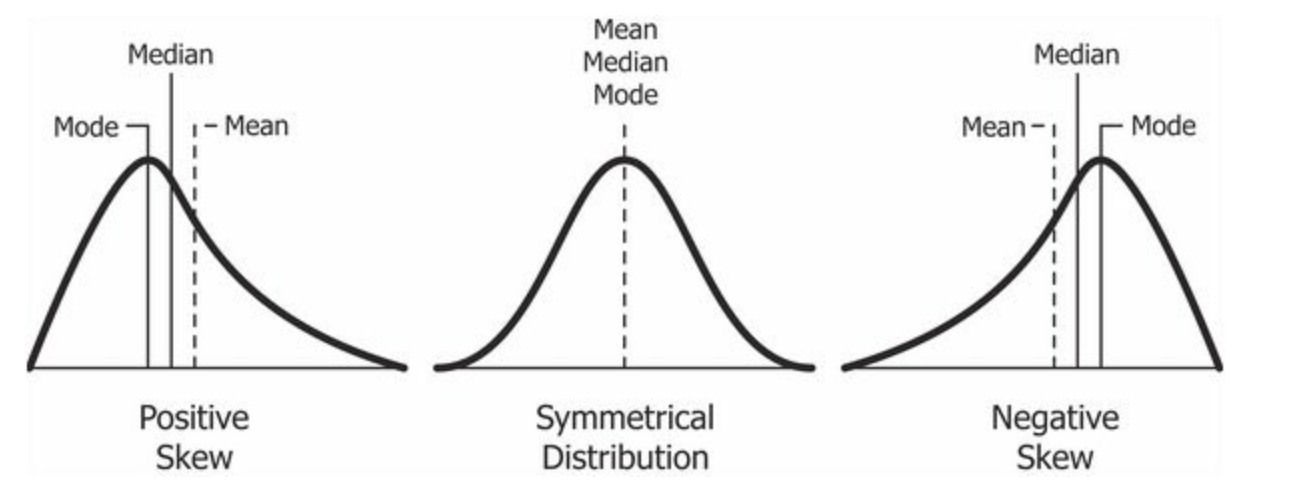
\includegraphics[scale=0.8]{lit_review/skewness.png}
      \caption{Skewness Visualisation}
      \label{skewness fig}
      \emph{Source: Wikipedia}
\end{figure}

\subsubsection{Kurtosis}

Kurtosis is a measure of whether a sample is heavily tailed or lightly tailed relative to a normal distribution. A high kurtosis value infers that a data set will have a large amount of outliers. On the other hand a low kurtosis value indicates a data set with very few outliers. The kurtosis for a standard normal distribution is 3, hence a metric often used is referred to as the "excess kurtosis" and takes the value $kurtosis - 1$.

Mathematically, the kurtosis value is calculated as such:
\begin{equation}
    kurtosis = \frac{1}{N - 1} \frac{\sum_{i=1}^{N}(x_{i} - \bar{x})^{4}}{S^{4}}
\end{equation}

\subsubsection{P-Value}

The P-Value is used in null hypothesis significance testing. Assuming a null hypothesis $H_{0}$, a hypothesis of no difference, and a second hypothesis $H_{1}$, representing the opposite of the null hypothesis. The P-Value is the probability of finding greater results when the null hypothesis $H_{0}$ is true. A level of significance is picked, typically one of 0.1, 0.05 or 0.01. A p-value below the threshold, then we can conclude that there is significant evidence to reject the null hypothesis $H_{0}$. This study uses a significance level of 5\% (p-value of 0.05) by default unless specified otherwise.

\subsubsection{Correlation}

This study makes use of the Pearson product-moment correlation coefficient. Correlation (r) quantifies linear relationship between two data sets. Its values ranges between -1 and 1. A correlation value of zero indicates no linear relationship between the two sets of data. A positive correlation indicates that both variables move in the same direction, it shows that when one becomes larger or smaller, so does the other. On the other hand, a negative correlation shows the opposite: both variables move in the opposite directions. 
A larger distance between zero and the correlation value indicates a stronger relationship, this is true for both positive and negative correlations. The coefficient can be computed using the formula below.

\begin{equation}
    r = \frac{\sum_{i=1}^{N}(x_{i} - \bar{x})(y_{i} - \bar{y})}{\sqrt{\sum_{i=1}^{N}(x_{i} - \bar{x})^{2}\sum_{i=1}^{N}(y_{i} - \bar{y})^{2}}}
\end{equation}
Note that both sets of data must be of the same size. Here N is the sample size of both x and y data sets, $x_{i}$ and $y_{i}$ are the ith data point for data sets x and y respectively, finally $\bar{x}$ and $\bar{y}$ are the means for both data sets.

\subsubsection{Z-Score}

The Z-Score (Z), also known as the standard score, is a value which shows a measure of the a value's relationship to the mean of the data set it belongs to. It represents the number of standard deviations by which a value is above or below the mean value.

\begin{equation}
    Z = \frac{x - \bar{x}}{S}
\end{equation}
Where x is a value of the data set, $\bar{x}$ is the mean and $S$ is the standard deviation.

\subsection{TODO: VAR / Causality Test}
TODO
%- main statistical measures
%- correlation 
%- statistical significance (look into durbin watson), hypothesis testing
%- F-statistic with p-value
%- unit root test
%- R\^2
%- granger causuality test
%- VAR ?
%- variance, z-score

\chapter{Method}\label{Method}

This section will go through an overview of the design choices that were made throughout this project on various levels in order to ultimately achieve the previously laid out research objectives (Chapter \ref{Introduction}). These design choices can be grouped into three different categories: Data Gathering, Sentiment Analysis and Statistical Analysis. Each of which will be explained in detail in the paragraphs below. An overview of the entire system can be found in Figure \ref{system figure}.


\begin{figure}[h!]
      \centering
      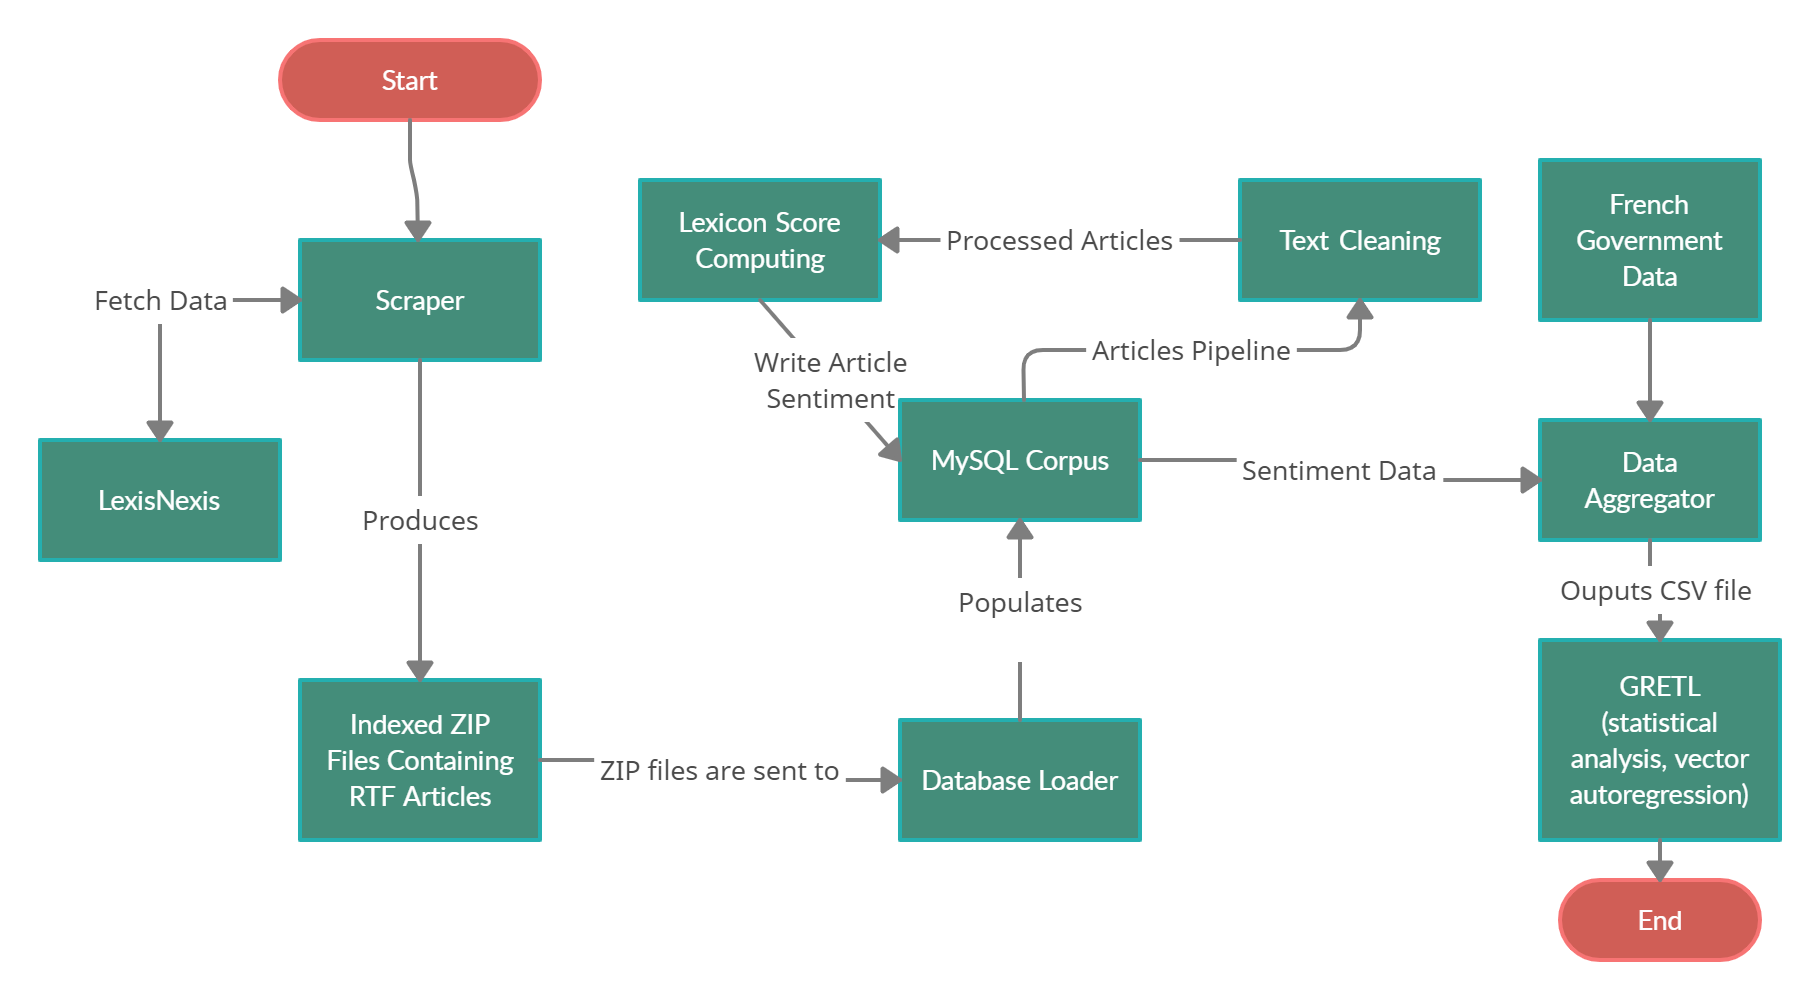
\includegraphics[scale=0.23]{method/system.png}
      \caption{System Overview}
      \label{system figure}
\end{figure}

\section{Data Gathering}

The first part of this subsection addresses the process of identifying, gathering and organising data such as to create a quality corpus and to achieve the research objective: \emph{Gather a large corpus containing high quality French news articles relevant to COVID-19}.

\subsection{Relevant Articles Of Quality}

This section provides answers to the following questions about creating this data set:
\begin{enumerate}
    \item What makes an article relevant for the corpus?
    \item How to ensure the quality of the corpus?
    \item When should the start and end date for data collection be?
\end{enumerate}

\subsubsection{Relevancy}

An important part of gathering data is making sure of the data's relevancy, which validates that the corpus to be built will be ultimately useful and for the results to be relevant. In order to build a relevant corpus, articles must show relevance to COVID-19. To verify an article's relevancy, the mention of "covid", "corona", "COVID-19" or "coronavirus" in an article is sufficient to label an article as relevant.

A second variable important to building this corpus is timing. Articles are only relevant if they occured within the time window of the COVID-19 pandemic. According to the WHO\footnote{\url{https://www.who.int/news/item/29-06-2020-covidtimeline}}, the first COVID-19 event worldwide dates from the 31st of December 2019. The corpus was built using a time range from the 1st January 2020 until the 25th March 2021 which is the date when data collection was finished. It may look at first like the 31st December 2019 should have been included in the range, it turns out that the data shows the first month of events was not reported much in french news articles, in fact it represents less than $0.005\%$ of the articles in the corpus with the first article being published on the 2nd of January 2020 and the second one on the 10th.

Final details to ensure relevancy include making sure that the publication language is in french as well as the publication location to be in France.

\subsubsection{Quality Articles}

A large amount of articles are written continuously on many different platforms such as social media, news platforms or web blogs for example. This study will focus on french news articles as they play a major role in distributing information to the general public. The Alliance pour les chiffres de la presse et des médias (ACPM)\footnote{\url{https://www.acpm.fr/Les-chiffres/Observatoire-2020-de-l-ACPM-Syntheses-2019}} is a non-profit organisation which verifies the distribution of french newspapers. The ACPM recorded an average of 9 million physical articles diffused and 60 million online visits daily in their 2020 review. To put these numbers into perspective, the Institut national de la statistique et des études économiques (INSEE)\footnote{\url{https://www.insee.fr/fr/statistiques/1892117?sommaire=1912926}}, the national statistics bureau of France, recorded a total population of 67 million in 2020. Studying these articles is thus particularly interesting given the large fraction of the population who are reading them. It is also worth noting that articles published by reputable sources are written by professionals, fact checked and verified on multiple levels within a news organisation before getting published. By targeting reputable french news sources, it is then expected to obtain a corpus containing high-quality, professionally written articles. It is important to make sure that any selected source is of sufficient quality as outlined above. Because of this, online blogs and sites have not been included in the corpus as they do not meet the quality threshold. These sources have been found to heavily reference themselves and rely on other news sources \cite{adamic2005political}. To further ensure quality, the sources of this corpus have all made a licensing agreement with LexisNexis News \& Business.

\subsubsection{Duplicates}

Methods were originally put in place to identify and remove duplicate articles by computing a ratio of similarity. After some considerations duplicate articles were kept in the corpus for multiple reasons.

Firstly, it is worth clarifying what is meant by duplicate articles: an article that has been published by a individual source will not be included twice in the corpus. Duplicates here are articles that may be published multiple times by different sources. For example a news organisation may be publishing multiple regional news editions which may include the same or a slightly modified version of the same content. Hence while one original writing was published multiple times, it was done so by different sources.

By keeping those duplicate articles, the corpus represents more accurately the flow of information being made available to the public by news organisations. The repetition of a story in different sources reflects its importance and not including articles from certain sources because of a duplicate article would bias any source-specific analysis.

Doing so removes the need for deduplication which is a challenge of its own. News articles are rather large in nature and computing string similarity ratios for each pair of articles can be very expensive to compute.

\subsection{Large Data Collection}\label{Data Collection}

With regards to how big the corpus should be, there are three questions to answer:
\begin{enumerate}
    \item How many articles should be gathered?
    \item How many articles should be retrieved per source?
    \item How to gather articles and structure the corpus?
\end{enumerate}

\subsubsection{Corpus Size Assessment}

It is important to build a corpus of a substantial size such as to avoid any potential biases which can occur with small sample sizes. It is also important to include both national and regional publications. While some types of regional publications consist mostly of national news, most regional publications are found to differ significantly in content when compared to national publications \cite{ballarini2008presse}. France is home to hundreds of different news sources, when considering all the different type of news publications such as daily, weekly, biweekly, monthly and more. Over 200 of which have business agreements with LexisNexis News \& Business. This makes for a sufficient selection of sources for this corpus.

With regards to the quantity of articles to gather per source, the goal is to retrieve as many articles per source matching the relevancy criteria. LexisNexis makes it possible to retrieve all of the articles matching the relevancy criteria for the selected sources which removes the need of selecting a random sample. This will enable analysis on which sources publish the most COVID-19 related articles as well as the variations in the amount of articles published over key events or periods. It is worth noting that this may introduce a bias in other analyses as some sources publish much more than others, it remains however necessary for the corpus built to be large enough.

To summarize, the corpus will be built by gathering as many articles as possible that match the relevancy criteria and come from a set of selected sources. As many sources as possible will be selected, given that they match the quality standard discussed above and have a licensing agreement with LexisNexis \& Business.

\subsubsection{Collecting Data}\label{Collecting Data}

A small corpus was originally built by manually downloading articles matching the previously laid out relevancy filters from LexisNexis, it quickly became apparent that such an approach would not be sufficient to build a corpus large enough for this study.

A scraper was built instead to automate the process of downloading those articles. A total of 369,569 articles listed on LexisNexis match the selected filters. As a service, LexisNexis enables downloading articles in batches of up to 500. It also enables options into the formatting of documents such link embedding, text formatting and more. As part of this system, the documents will be downloaded in rich text format (RTF), references will not be embedded as links such as to simplify the document parsing process, and articles will be saved as individual files which will be compressed as a ZIP file grouping 500 articles each. Note that all of these are options to be set by the scrapper on the options dialog before triggering a download.

The technologies used to build the scraper include the Google Chrome browser, its associated "ChromeDriver" which enables triggering browser actions programmatically, the Python programming language and finally Selenium. Selenium is an open-source framework which makes performing automated browser actions easier.

Here is a simplified overview of the actions performed by this scraper in pseudo code:

\begin{verbatim}
load_url()
login()
handle_pop_ups()
while !finished_downloading() {
    open_download_dialog()
    enter_download_parameters()
    trigger_download()
    wait_for_download_triggered()
    wait_for_download_finished()
    rename_and_index_downloaded_file()
}
\end{verbatim}

There were a few issues specific to LexisNexis that needed solving before having a working, independent scraper. The first one was dealing with pop-ups. Opening LexisNexis from a scrapper with no cookies will open 0 to 3 different pop-ups promoting various events. To avoid scrapers these pop-ups include an automatically generated id in their HTML tag which made it harder to close automatically, their load time varied heavily as well. To solve this issue, a time period of 60 seconds on page load was put in place. During that time the system attempts to identify any pop-up HTML component and identify any buttons within the component. Such pop-ups only include close buttons which made the closing task easier.

Another issue that was later discovered is that downloading articles from LexisNexis requires a range of articles to download, for instance a range of 1-500 would download the first 500 articles matched. The issue came when using an offset greater than 30,000 (for example a range of 30,001 - 30,500) which broke LexisNexis' download system and no download would be triggered. To solve this issue, batches of a maximum of 30,000 articles were created manually. The process for doing so was:
\begin{enumerate}
    \item Manually log into LexisNexis and set the search filters.
    \item Select a time range such that the total returned articles is below 30,000.
    \item Copy a permanent link URL such that the scraper can load load the URL with the filters and time range already set. Also copy the total number of articles.
    \item Repeat the process such that the whole time range is covered. It is very important to make sure not to include date overlaps as doing so would introduce duplicate articles.
\end{enumerate}

From this process a set of URLs as well as their associated article counts are obtained. The scrapper can now iterate through these batches and download all the targeted articles.

Another issue the scrapper ran into was rate limiting. The university limits how many downloads one account can make over a certain period of time. When that limit is reached, the account is blocked from accessing LexisNexis for two hours. The only solution for this was to have the scraper identify the rate-limiting web page and to let the script sleep for two hours when the event occurs.

Finally, it was crucial for the scrapper to be able to handle unexpected errors gracefully. Given that it was executed for a time period of 7 days in total, unexpected network errors and many others could occur. Hence before starting to download articles, a check is performed in the directories containing previously downloaded files such as to identify which batches are complete and which ones are not. That way the scraper can resume work where it left off in case of any error.

Running this system for a week was sufficient for the system to download all of the 369,569 articles that matched the previously selected set of filters.

\subsubsection{Organising Data}

This section will include details as to how the scraper system organises downloaded files as well as how the downloaded articles were aggregated to enable easy and fast operations.

Once a download finished successfully, the scrapper moves that file from the download directory to the output directory matching the current batch of articles being downloaded. The output directories include all of the indexed files that were previously downloaded. When moved to an output directory, the files are renamed to include information about the batch they come from as well as the offset used to obtain this file. This indexing enables the scraper to keep track of which files have and haven't been downloaded, hence making sure that no individual article is downloaded twice.

The next task is to extract relevant information from the 740 ZIP files, containing 369,569 individual articles that were downloaded by the scraper. A MySQL database was used to organise the corpus as it enables easy and fast operations that wouldn't be possible otherwise.

The process of loading the data into a structured, relational database also required important design choices. Similar to the scrapper, care must be placed in loading each article no more than once, and, given the amount of data to be handled, the system must be able to resume work on error. The procedure for loading data is detailed in Figure \ref{database loader}. The approach writes important data to text files to keep track of which ZIP file is currently being processed and a separate file to keep track of the list of ZIP files which have been already loaded. By doing so the system knows at all times what work has been done and what is remaining, hence enabling the system to crash and resume work where it left off. The final detail is that after a specific RTF file containing a single article was parsed and loaded into the database, that file is deleted to make sure not to load it twice.

\begin{figure}[h!]
      \centering
      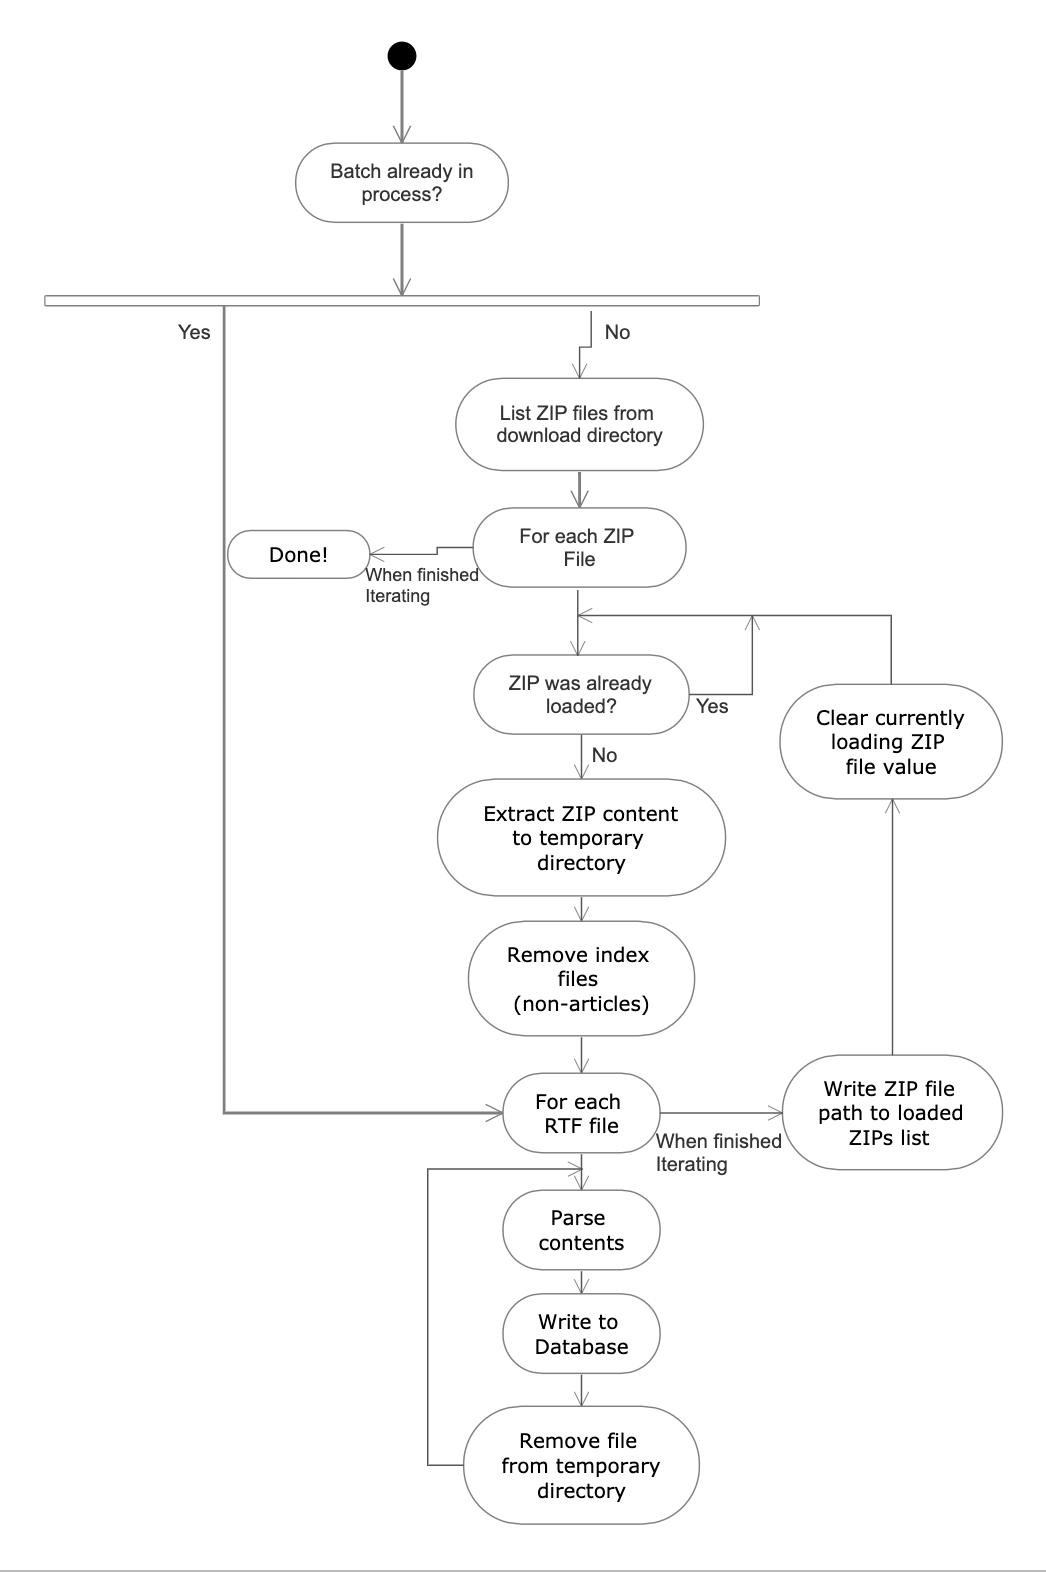
\includegraphics[scale=0.7]{method/Screenshot 2021-04-19 at 15.12.36.png}
      \caption{Loading Articles Into a MySQL Database Pipeline}
      \label{database loader}
\end{figure}

Finally, the articles come in rich text format (RTF). The content parsing algorithm parses and splits the RTF text into various sections:
\begin{enumerate}
    \item Article title
    \item Source
    \item Date
    \item Copyright
    \item Body
    \item Author
\end{enumerate}

More information is extracted however the above fields represent the most important data points to be used throughout this study. To conclude this section, it is worth noting that a number of articles did not include a date, or was formatted differently than the parser expected. In these instances, the article was not loaded into the database as the timing of an article was deemed important to this study.

\section{Sentiment Analysis}

The following subsection will cover the sentiment analysis part of this study. Including both the dictionaries used as well as the sentiment analysis pipelines. It addresses the following two research objectives: \emph{Create specialised dictionaries targeted to measure pandemic-related sentiments} as well as \emph{Perform sentiment analysis on the corpus to retrieve measures for various sentiments and term frequencies}.

\subsection{Specialised Dictionaries}\label{Custom Dicts}

In order to extract information specific to the COVID-19 pandemic, three specialist dictionaries were created. These dictionaries target the mentions of virus, vaccination and death. The process for creating these three dictionaries involved the corpus analysis tool AntConc\footnote{\url{https://www.laurenceanthony.net/software/antconc/}}. AntConc enables the analysis of word patterns within a corpus, a manual selection of terms from the analysis performed in AntConc yielded the three dictionaries.

Finally, it is worth noting that all three dictionaries consist of word lemmas, stop words have been removed and all of the terms were mapped to lowercase.

\subsubsection{Virus}

The Virus dictionary is the largest out of the three as it is also the most vast. The aim of this lexicon is to enable the measurement of virus-related words. It consists of words, expressions and objects that have been made popular or used in the context of the COVID-19 pandemic. The total lexicon includes seventy five words, Table \ref{tab:virus lexicon} shows twenty five entries. Care was put in reducing overlap between the three dictionaries, since this one was the largest, death and vaccination related terms have not been included in this lexicon.

\begin{table}[htb]
\caption{Virus Lexicon}
\label{tab:virus lexicon}
\centering
\csvautobooktabularcenter{method/virus_lexicon.txt}
\end{table}

\subsubsection{Vaccine}

Similarly, this lexicon aims to quantify the presence of vaccination-related words in articles. It consists of twenty eight words which are displayed in Table \ref{tab:vaccine lexicon}. The words included consist of a lexicon around vaccination as well as the names of the available COVID-19 vaccines or companies producing them.

\begin{table}[htb]
\caption{Vaccine Lexicon}
\label{tab:vaccine lexicon}
\centering
\csvautobooktabularcenter{method/vaccine_lexicon.txt}
\end{table}

\subsubsection{Death}

This final lexicon targets the mention of death within an article, it consists of sixty five words in total, twenty five of which are shown in Table \ref{tab:death lexicon}.

\begin{table}[htb]
\caption{Death Lexicon}
\label{tab:death lexicon}
\centering
\csvautobooktabularcenter{method/death_lexicon.txt}
\end{table}

\subsection{Sentiment Analysis Pipeline}

Originally the text analysis software Rocksteady \cite{ahmad2014rocksteady} was used. Rocksteady is a lexicon based affect analysis system which was developed in Trinity College Dublin, Ireland. Once the scraper system (Chapter \ref{Collecting Data}) was put in place it became apparent that a more flexible system was required. Rocksteady requires the aggregation of articles into text files which comes with limitations, handling 369,569 articles in the form of text files is very expensive, whether it is to aggregate the corpus into a single or many files such that Rocksteady can read the corpus, reading all of that data on each load, computing all of the sentiments for the whole corpus at once which could run into memory issues as attempting to compute sentiment for a large amount of articles requires a flexible system such that sentiment can be computed through a data pipeline. In light of this, the articles were parsed, organised and loaded into a MySQL database as described in Chapter \ref{Collecting Data}. This system also enables extremely fast article retrieval as well as very useful data aggregation methods such as date grouping, source grouping and more within seconds. The following sections explain in detail how the system was implemented.
 
\subsubsection{Lexicon Handling}

The first part of performing lexicon based sentiment analysis on an article is to first load and process the various lexicons used. As part of this project three specialist dictionaries (Chapter \ref{Custom Dicts}) were used. FEEL, Diko as well as Polarimots (Chapter \ref{French Lexicons}) are three other lexicons which were used to measure polarity as well as other emotions where possible.

With regards to the custom dictionaries, the process for loading each lexicon was to load the text file containing the lexicon. These lexicons are built in the form of one word per line. Splitting the resulting string using the new line character yields an array of all of the words within that lexicon. No weight was associated for each of the words so the count of occurrences within an article was used as the final score for each lexicon.

FEEL, Diko and Polarimots required more processing. Each of these lexicons had specific requirements when it came to putting it into practise as some included specific emotions and details. The following sections will explain how weights were applied for each of these dictionaries.

The FEEL lexicon includes for each word a polarity (negative or positive) as well as a value of 1 or 0 for the following emotions: joy, fear, sadness, anger, surprise and disgust. For this lexicon a similar approach to the custom dictionaries was used: a count of occurrences for each of the emotions as well as the polarity occurrences.

The Diko Lexicon includes for each word a number of vote for its polarity (negative, positive, neutral). These numbers were used to compute a score for each word, the following points were taken in consideration:
\begin{enumerate}
    \item Amount of total votes relative to the entire lexicon
    \item Positive / negative vote frequency
    \item Neutral votes: a large number of neutral votes pushes the score towards 0
\end{enumerate}
To do so, the following value is computed:
\begin{equation}
    \frac{\#pos - \#neg}{\#pos + \#neg + \#neut}
\end{equation}
This scoring system works as it reflects the positive or negative frequency of votes relative to the total amount of votes. It is also important that more positive votes yields a positive score and on the contrary a negative score which is the case with this function. However it does not reflect an accurate score with regards to how many votes were observed relative to the entire lexicon. For example, a word with 10\% of positive votes, 80\% negative and 10\% neutral will have the same score if it has a total vote count of 10 or 10000. This needs to be taken into account as a reliability measurement.
To do so, we start by computing the Z-Score for the total vote counts, which measures how far apart from the mean a data point is:
\begin{equation}
    \frac{(\#pos + \#neg + \#neut) - \mu}{\sigma}
\end{equation}
Where $\mu$ is the mean for total votes on the lexicon and $\sigma$ is its standard deviation. This measure provides a reliability metric as previously discussed, however it comes with the issue of returning a negative value when the total word count is below the mean which is an issue for the final score. By not subtracting the mean in the Z-Score and multiplying both measures together, we obtain the weight function for this dictionary:
\begin{equation}
\label{diko score}
    score = \frac{\#pos - \#neg}{\#pos + \#neg + \#neut} * \frac{(\#pos + \#neg + \#neut)}{\sigma}
\end{equation}
Where $\#neg$, $\#neut$ $\#pos$ is the number of negative, neutral and positive votes respectively for a word entry, $\sigma$ is the standard deviation for total votes in the lexicon.

One final detail is that the Diko dictionary is very large, containing over 1.2 million word entries. Using the entire dictionary is not of much use and unrealistic on a large corpus. To do so, words with a total vote count below 500 were skipped as well as words with scores in the range of $-1 < score < 1$. This returns a total of 24,643 words to use from this lexicon.

Last but not least, the Polarimots dictionary includes for each word a polarity which can be one of neutral, positive and negative. Also associated with each word is a reliability metric of either 100\% 66\% or 33\%. This reliability metric was divided by 100 such as to obtain 0.33, 0.66 and 1 which makes for the weights used with this dictionary.

\subsubsection{Data Pipeline}

Given the large quantity of articles in this corpus. A data pipeline feeding articles to the sentiment analysis system is required such as not to load all of the articles at once. Articles are loaded in batches of 2000, once a batch is finished processing the resulting sentiment computed is saved into the database. The algorithm then ends once all of the articles sentiments have been saved to the database.

It was very important to save sentiment outputs to the database for two main reasons:
\begin{enumerate}
    \item Computing sentiment on the corpus for each lexicon took between 10 to 16 hours depending on the size of the lexicon used. Being able to proceed by batch and resume on error is valuable.
    \item Storing sentiment values in an articles metadata enables further analysis grouping or filtering articles within seconds by using the already computed sentiment values.
\end{enumerate}

\subsubsection{Text Cleaning}

Articles are put through a series of steps that modify them in some way in order to apply sentiment analysis to it in the best of conditions. First, the articles are converted to lowercase, this step is not always necessary but the lexicons used all use lowercase words. The second step is to remove stop words and punctuation. The list of stop words used come from SpaCy's french language pipeline (Chapter \ref{lemmatization}). Finally, the remaining words are lemmatized also using SpaCy.

\subsubsection{Computing Sentiment}

This final step receives a processed and cleaned text and outputs a set of sentiment scores. The first step to do so is to count the occurrences of the lexicon words within the article. While originally a set of nested for loops were put in place to do so. After some brief manual experiments, using regular expressions was found to be much faster. Hence from a provided lexicon, a single regular expression is compiled. The regular expression matches the following pattern:
\begin{center}
\begin{verbatim}(\bhello\b|\bworld\b)\end{verbatim}
\end{center}

The parentheses mark the group of the regular expression, the above expression would match the words "hello" and "world". Notice that they are wrapped in $\backslash$ followed by "b", this operator in regular expressions makes sure to only match entire words, hence making sure that a white space character is present before and after the word within the article. The final detail is that all of the lexicon's words are separated by a "|" operator which is the equivalent of the "OR" operation in a regular expression.

Using a lexicon's compiled regular expression as described above, we obtain a set of paired values, including a subset of the lexicons words and its associated number of occurrences within the article.
All that is left is to iterate through those matches, for each word retrieve the associated weight, make sure to multiply it by the number of occurrences and keep a running total of all of the sentiments included within the lexicon used.

Some sentiments systems will act as a classifiers, whether it is machine learning or lexicon based, by returning "positive" or "negative" for a specific article. This system does not and keeps both the positive and negative scores obtained from an article, it provides more details useful to the statistical analysis.

\subsection{Output Aggregating}\label{chap: output aggregating}

The final step of the sentiment analysis system is to format the output such that it can be used for a statistical analysis. To do so, information about the corpus as well as its computed sentiment scores are grouped daily and retrieved from the database. Official data from the french government\footnote{\url{https://www.data.gouv.fr/en/datasets/donnees-relatives-a-lepidemie-de-covid-19-en-france-vue-densemble/}} is appended to the sentiment data. Metrics used from the french government include: the number of confirmed COVID-19 cases, number of deaths and the number of first vaccine injections, corresponding to the data points "casConfirmes", "deces" and "nouvellesPremieresInjections" respectively in the summary data set.

\section{Statistical Analysis}

This final subsection of this chapter will cover details of the last remaining research objective: \emph{Conduct statistical analysis on the results in order to identify and quantify potential relationships}.

\subsection{TODO}
\chapter{Experiments and Results}\label{Evalutation}

This chapter introduces the results obtained from the steps detailed in the previous chapter. It begins with a discussion and an overview of the corpus collected. Then, a section presenting sentiment analysis as well as the frequency of term mentions within the previously created specialist dictionaries (Chapter \ref{Data Collection}). Finally, a statistical analysis will be performed such as to identify any potential relationship between the presented variables. 

\section{Data Collection}

From the original 369,569 articles downloaded using the approach detailed in Chapter \ref{Collecting Data}, a total of 305,454 were loaded into the database after date and source filtering was performed, removing a total of 17.34\% of articles. Table \ref{tab: corpus size} includes key information with regards to  the size of the corpus. The selected period makes for a total of 450 days, the average daily article count is then of 679 articles per day. Table \ref{tab:core stat source} and Table \ref{tab:stat source} include core statistics relating to sources, on average individual sources contain 1351.57 articles with a very high standard deviation of 3220.96 which shows that the data is heavily dispersed, as we can see looking at the minimum and maximum article count per source, 1 and 30,767 respectively, we can clearly see how that can be the case. Furthermore, as previously explained (Chapter \ref{Statistical Methods}), the skewness measures the distribution of articles, 5.61 is considered a high value which signifies that the data is heavily skewed to the right, meaning that the right side of the distribution is longer. This is confirmed by the high kurtosis value of 40.31, showing a high amount of outliers in our data distribution, confirming the above analysis.

Table \ref{tab:stat source} displays metrics about the thirty largest sources, it is found that while five sources have over 10,000 articles, it quickly drops with the last few sources showing article counts closer to 3,000 which is much closer to the observed mean.

Looking at the largest source, \emph{Agence France Presse} (AFP), its details have been previously discussed (Chapter \ref{chap:French Press}). The following sources are part of the largest French news organisations so it comes as no surprise that their article count is very high.

Analysing the sources with the least amount of articles, it is found that 158 sources have less than 1000 articles and 104 have less than 200. Considering that the total number of selected sources is 226, the majority are found to contain a number of articles significantly lower than the mean as the counts are quite dispersed. Digging deeper, it is found that some sources appear under different names, for instance, Table \ref{tab:source repetition} shows an example of one source appearing under many different regional editions. This is occurs in many times within the corpus which explains how the sources are so spread out. 

\begin{table}[H]
\centering
\begin{tabular}{lll}
\toprule
Sources & Articles & Words \\ \hline
226 & 305,454 & 167,800,491 \\
\bottomrule
\end{tabular}
\caption{Corpus Size}
\label{tab: corpus size}
\end{table}

\begin{table}[H]
\centering
\begin{tabular}{@{}lllllll@{}}
\toprule
 & Mean & Std Dev & Skewness & Kurtosis & Minimum & Maximum \\ \midrule
Articles per Source & 1352 & 3221 & 6 & 40 & 1 & 30,767 \\ \bottomrule
\end{tabular}
\caption{Article Statistics Overview}
\label{tab:core stat source}
\end{table}

\begin{table}[H]
\caption{Example of Source Repetition}
\label{tab:source repetition}
\centering
\begin{tabular}{l}
\toprule
\emph{20 Minutes} \\
\emph{20 Minutes Bordeaux} \\
\emph{20 Minutes Lille} \\
\emph{20 Minutes Lyon} \\
\emph{20 Minutes Marseille} \\
\emph{20 Minutes Montpellier} \\
\emph{20 Minutes Nantes} \\
\emph{20 Minutes Nice} \\
\emph{20 Minutes Paris} \\
\emph{20 Minutes Rennes} \\
\emph{20 Minutes Strasbourg} \\
\emph{20 Minutes Toulouse} \\
\bottomrule
\end{tabular} \\[0.2cm]
Some sources appear under different names in the corpus, this causes for the data as observed in Table \ref{tab:core stat source} to be spread out.
\end{table}

\begin{table}[H]
\caption{Article Breakdown Per Source}
\label{tab:stat source}
\resizebox{\textwidth}{!}{%
\begin{tabular}{@{}|crrr|@{}}
\toprule
\textbf{Source (First 30)} & \multicolumn{1}{c}{\textbf{Article Count}} & \multicolumn{1}{c}{\textbf{Word Count}} & \multicolumn{1}{c|}{\textbf{Mean Words}} \\ \midrule
\emph{Agence France Presse} & 30767 & 14808082 & 481 \\
\emph{Lefigaro.fr} & 21978 & 12111314 & 551 \\
\emph{Le Dauphiné Libéré} & 17888 & 6334269 & 354 \\
\emph{Le Progrès} & 11424 & 4345194 & 380 \\
\emph{Challenges.fr} & 11139 & 6740282 & 605 \\
\emph{La Depeche du Midi} & 9687 & 3750146 & 387 \\
\emph{LesEchos.fr} & 8801 & 7457331 & 847 \\
\emph{La Nouvelle République du Centre Ouest} & 7180 & 2504550 & 349 \\
\emph{Le Télégramme} & 6853 & 2140967 & 312 \\
\emph{La Montagne} & 5625 & 2042911 & 363 \\
\emph{L'Est Républicain} & 5529 & 1960041 & 355 \\
\emph{Les Echos} & 5212 & 3291085 & 631 \\
\emph{Vosges Matin} & 4754 & 1722946 & 362 \\
\emph{MIDI LIBRE} & 4719 & 1717583 & 364 \\
\emph{Le Figaro} & 4712 & 3188302 & 677 \\
\emph{Courrier de l'Ouest} & 4645 & 1573221 & 339 \\
\emph{Le Figaro Économie} & 4556 & 3094663 & 679 \\
\emph{Sciences et Avenir.fr} & 4539 & 3316758 & 731 \\
\emph{L'Obs} & 3649 & 2798011 & 767 \\
\emph{Nice Matin} & 3453 & 2744343 & 795 \\
\emph{Le Courrier Picard} & 3356 & 1306574 & 389 \\
\emph{Le Républicain Lorrain} & 3346 & 1222386 & 365 \\
\emph{L'INDEPENDANT} & 3276 & 1100647 & 336 \\
\emph{La Tribune} & 3049 & 2782505 & 913 \\
\emph{LePoint.fr} & 2923 & 2909518 & 995 \\
\emph{L'Est-eclair - Liberation Champagne} & 2914 & 1100477 & 378 \\
\emph{Le Petit Journal} & 2860 & 830362 & 290 \\
\emph{FRANCE 24 (French)} & 2806 & 1733556 & 618 \\
\emph{Var Matin} & 2761 & 1996749 & 723 \\
\emph{La Tribune.fr} & 2732 & 2405697 & 881 \\
\emph{Le Berry Républicain} & 2718 & 1067047 & 393 \\ \bottomrule
\end{tabular}%
}
\end{table}

\section{Sentiment Analysis}

\subsection{Polarity Analysis}

Looking at the scores for polarity on the corpus as shown in Table \ref{tab:dict stats}, means and standard deviations for the three dictionaries are found to be quite different, that is simply because they each use a specific weighting system. The following results will focus on the output of FEEL (Chapter \ref{chap: feel}) as it also includes sentiment for a set of emotions such as fear, joy and more and, like the specialised dictionaries, its weighing system simply count word occurrences. An overview of the sentiment scores can be found in Table \ref{tab:feel stats}, given that FEEL counts the number of matched terms for each category, scores have been converted to percentages of the articles lengths such as to make these numbers easier to understand. 

We find that positivity and negativity occur the most often in the corpus (23\% and 6.2\% on average respectively) with other emotions representing a range between 1.12\% to 4.63\% of all terms on average. Positivity, negativity and fear are considered "relatively symmetric" looking at the skewness value, on the other hand, joy, sadness, anger, surprise and disgust are found to be highly skewed. The kurtosis measure for most of these measures are found to be relatively close to the normal distribution, with the exception of joy (5.32) and surprise (9.16) which have high kurtosis values indicating that these distributions have a large amount of outliers.

\begin{table}[H]
\centering
\begin{tabular}{@{}|c|llll|@{}}
\toprule
 & \multicolumn{1}{c}{\textbf{Mean}} & \multicolumn{1}{c}{\textbf{Std Dev}} & \multicolumn{1}{c}{\textbf{Min}} & \multicolumn{1}{c|}{\textbf{Max}} \\ \midrule
\textbf{FEEL Positive} & 0.230 & 0.034 & 0.000 & 0.500 \\
\textbf{FEEL Negative} & 0.062 & 0.022 & 0.000 & 0.309 \\
\textbf{Polarimots Positive} & 0.014 & 0.007 & 0.000 & 0.102 \\
\textbf{Polarimots Negative} & 0.004 & 0.004 & 0.000 & 0.105 \\
\textbf{Diko Positive} & 0.395 & 0.068 & 0.000 & 2.498 \\
\textbf{Diko Negative} & 0.144 & 0.084 & 0.000 & 1.647 \\ \bottomrule
\end{tabular}
\caption{Dictionaries Sentiment Comparison}
Values were converted to be relative to the corpus size and absolute.\\Values represent individual articles with no grouping.
\label{tab:dict stats}
\end{table}

\begin{table}[H]
\centering
\begin{tabular}{@{}ccccc@{}}
\toprule
         & Mean    & Std Dev & Skewness & Kurtosis \\ \midrule
Positive & 22.98\% & 3.36\%  & -0.17  & 2.55   \\
Negative & 6.18\%  & 2.18\%  & 0.50   & 1.30   \\
Joy      & 1.12\%  & 0.75\%  & 1.48   & 5.32   \\
Fear     & 4.63\%  & 1.84\%  & 0.63   & 1.64   \\
Sadness  & 3.81\%  & 1.72\%  & 0.92   & 2.63   \\
Anger    & 2.43\%  & 1.32\%  & 1.10   & 3.34   \\
Surprise & 2.26\%  & 1.14\%  & 1.31   & 9.16   \\
Disgust  & 1.81\%  & 1.12\%  & 1.20   & 3.61   \\
\bottomrule
\end{tabular}
\caption{FEEL Sentiment Overview}
\label{tab:feel stats}
\emph{Values represent individual articles with no grouping.}
\end{table}

\subsection{Virus Mentions}

The virus dictionary is the largest of all three so it is no surprise that within the dictionary, the mean rate of mentions per word is of 1.39\% and the standard deviation is of 3.18\%. The mean and standard deviation show that a select set of words represent most of the mentions. This is confirmed in Table \ref{tab:virus freqs} which shows the fifteen most mentioned terms over the corpus, clearly the first seven terms make up most of the mentions. In total, words of this dictionary have been found 2,250,684 times within the corpus which makes for a total of 1.34\% of all words within the dictionary.

\begin{table}[H]
\caption{Virus Dictionary Analysis}
\label{tab:virus freqs}
\centering
\begin{tabular}{@{}cc@{}}
\toprule
Word      & Proportion \\ \midrule
covid-19      & 19.45\% \\
coronavirus   & 10.92\% \\
pandémie      & 9.01\%  \\
confinement   & 8.43\%  \\
virus         & 7.98\%  \\
épidémie      & 7.96\%  \\
masque        & 6.62\%  \\
contamination & 2.68\%  \\
réanimation   & 2.42\%  \\
restriction   & 1.94\%  \\
dépistage     & 1.59\%  \\
infection     & 1.57\%  \\
déconfinement & 1.53\%  \\
symptôme      & 1.49\%  \\
contaminer    & 1.39\%  \\ \bottomrule
\end{tabular}
\end{table}

\subsection{Vaccine Mentions}

The vaccine dictionary has matched a total of 510,088 words in the corpus, in percentages this makes 0.30\% of the corpus. Within the dictionary, the mean rate of mentions is of 3.70\% and the standard deviation of 6.88\% hence the data is quite spread out. Once again, as shown in Table \ref{tab:vaccine freqs}, the first four words make up for 67\% of the entire dictionary mentions.

\begin{table}[H]
\caption{Vaccine Dictionary Analysis}
\label{tab:vaccine freqs}
\centering
\begin{tabular}{@{}cc@{}}
\toprule
Word      & Proportion \\ \midrule
vaccin      & 33.26\% \\
vaccination & 15.38\% \\
dose        & 10.10\% \\
vacciner    & 8.33\%  \\
pfizer      & 4.54\%  \\
astrazeneca & 4.19\%  \\
injection   & 3.11\%  \\
biontech    & 2.84\%  \\
anticorps   & 2.75\%  \\
moderna     & 2.41\%  \\
vaccinal    & 2.13\%  \\
immunité    & 2.13\%  \\
sanofi      & 1.77\%  \\
administrer & 1.67\%  \\
arn         & 1.05\%  \\ \bottomrule
\end{tabular}
\end{table}

\subsection{Death Mentions}

The death dictionary shows similar metrics to the vaccine dictionary. Its words were found a total of 527,011 times in the corpus, making for 0.31\% of the total corpus. The mean rate of mentions within the dictionary is of 1.56\% and the standard deviation of 4.52\%, once again showing a high value. Similarly, the rate of mentions is quite disproportionate, as shown in Table \ref{tab:death freqs}, the first four words make up for 73.77\% of the entire dictionary mentions.

\begin{table}[H]
\caption{Death Dictionary Analysis}
\label{tab:death freqs}
\centering
\begin{tabular}{@{}cc@{}}
\toprule
Word      & Proportion \\ \midrule
hôpital     & 22.21\% \\
mort        & 18.87\% \\
décès       & 17.32\% \\
maladie     & 15.37\% \\
victime     & 4.43\%  \\
décéder     & 3.87\%  \\
mourir      & 3.30\%  \\
tuer        & 2.25\%  \\
disparaître & 1.80\%  \\
mortel      & 0.95\%  \\
tombe       & 0.82\%  \\
disparition & 0.74\%  \\
cimetière   & 0.58\%  \\
exécution   & 0.56\%  \\
éteindre    & 0.55\%  \\ \bottomrule
\end{tabular}
\end{table}

\section{Statistical Analysis}

\subsection{Correlation}

Tables \ref{tab: correlation 1/2} and  \ref{tab: correlation 2/2} show an overview of the correlations found between the computed sentiment variables as well as France's COVID-19 epidemiology data provided by the French government\footnote{\url{https://www.data.gouv.fr/en/datasets/donnees-relatives-a-lepidemie-de-covid-19-en-france-vue-densemble/}} (Chapter \ref{chap: output aggregating}). Bold values are statistically significant with P < 0.05.

The number of daily articles is found to be positively correlated with the death count (0.50) as well as negativity, fear, sadness, anger and surprise, but is found to be negatively correlated with both virus and death sentiment. The number of new covid cases is found to be positively correlated with the number of daily death, vaccinations and new cases but is found to be negatively correlated with both virus and death sentiment, as well as joy, fear, surprise and disgust. Surprisingly, the number of daily deaths is not correlated with death sentiment. Instead it is found to be positively correlated with the vaccination rate and sentiment, as well as the average article length. It is also found to be negatively correlated with virus sentiment, joy and disgust. The daily vaccination rate is unsurprisingly found to be positively correlated (0.58) with vaccine sentiment, however, it is also negatively correlated with virus and death sentiment, as well as all of the FEEL recorded sentiments. It is surprising that positive terms are positively correlated with negative terms (0.62), in fact it is found that most of the FEEL recorded emotions are positively correlated. To finish, vaccine sentiment is positively correlated with death sentiment (0.63).

\begin{table}[H]
\centering
\resizebox{\textwidth}{!}{%
\begin{tabular}{|c|cccccccc|}
\hline
\multicolumn{1}{|l|}{} & ArticleCount & Cases & Death & Doses & VaccineDict & VirusDict & DeathDict & Length \\ \hline
ArticleCount &  &  &  &  &  &  &  &  \\
Cases &  &  &  &  &  &  &  &  \\
Death & 0.50 & 0.43 &  &  &  &  &  &  \\
Doses &  & 0.45 & 0.28 &  &  &  &  &  \\
VaccineDict &  & 0.44 & 0.48 & 0.58 &  &  &  &  \\
VirusDict & -0.21 & -0.29 & -0.15 & -0.26 & -0.19 &  &  &  \\
DeathDict & -0.13 & -0.28 &  & -0.22 & -0.25 & 0.63 &  &  \\
Length & 0.99 &  & 0.48 &  &  & -0.17 &  &  \\
Pos &  &  &  & -0.12 & 0.18 & 0.12 &  &  \\
Neg & 0.18 &  &  & -0.19 &  & 0.20 & 0.10 & 0.17 \\
Joy &  & -0.12 & -0.15 & -0.16 &  & 0.18 &  &  \\
Fear & 0.14 & -0.11 &  & -0.21 &  & 0.10 & 0.21 & 0.14 \\
Sadness & 0.18 & -0.14 &  & -0.29 & -0.15 &  & 0.13 & 0.18 \\
Anger & 0.35 &  &  & -0.16 &  & -0.16 & -0.10 & 0.33 \\
Surprise & 0.24 & -0.12 &  & -0.30 & -0.16 &  &  & 0.22 \\
Disgust &  & -0.19 & -0.10 & -0.18 &  & 0.26 & 0.16 &  \\ \hline
\end{tabular}%
}
\caption{Correlation Matrix of Sentiment and Government COVID-19 Epidemiology (Table 1/2)}
\label{tab: correlation 1/2}
Only statistically significant correlations with p < 0.05 are shown.
\end{table}


\begin{table}[H]
\centering
\resizebox{\textwidth}{!}{%
\begin{tabular}{|c|cccccccc|}
\hline
\multicolumn{1}{|l|}{} & Pos & Neg & Joy & Fear & Sadness & Anger & Surprise & Disgust \\ \hline
Neg & 0.62 &  &  &  &  &  &  &  \\
Joy & 0.50 &  &  &  &  &  &  &  \\
Fear & 0.59 & 0.88 &  &  &  &  &  &  \\
Sadness & 0.64 & 0.71 & 0.18 & 0.76 &  &  &  &  \\
Anger & 0.56 & 0.72 &  & 0.69 & 0.64 &  &  &  \\
Surprise & 0.61 & 0.55 & 0.26 & 0.51 & 0.69 & 0.71 &  &  \\
Disgust & 0.23 & 0.70 &  & 0.56 & 0.22 & 0.31 & 0.19 &  \\ \hline
\end{tabular}%
}
\caption{Correlation Matrix of Sentiment and Government COVID-19 Epidemiology (Table 2/2)}
Only statistically significant correlations with p < 0.05 are shown.
\label{tab: correlation 2/2}
\end{table}

\subsection{VAR Analysis}

A VAR analysis was performed on various models as defined previously (Chapter \ref{chap: stat analysis}). Models are built incrementally by adding one variable at a time and evaluating the results.

Firstly, variables are tested using the Augmented Dickey–Fuller test (ADF). This test checks that no unit root is present in each variable, hence making sure that the variables are stationary. In the case that the ADF test fails, variables are tested using the Engle Granger cointegration test. This test always failed in this experiment however had the test succeeded a vector error correction model (VEC) would have be used instead of a vector autoregression (VAR) model. Variables which failed the ADF test and the cointegration test were first-order differentiated. The selection of an optimal lag length is then performed by the use of the Akaike Information Criterion (AIC), Bayesian Information Criterion (BIC) and the Hannan-Quinn criterion (HQC). Finally, the resulting variables were added to the VAR model incrementally such as to quantify the differences each variable makes to the obtained model.

\subsubsection{Death Sentiment}

The variables for the number of deaths and cases failed both the ADF and cointegration tests. Their first-order difference has been used instead in this model as a result.

Table \ref{tab:model 1 lag} shows the results obtained for lag selection. We find that the three selection metrics all selected different length. BIC selected a lag of 1 which was ignored, secondly AIC selected lag 9 and HQC selected a lag of 7. Lag 9 was used in this instance as it was found to obtain superior results through manual testing.

\begin{table}[H]
\centering
\begin{tabular}{@{}llll@{}}
\toprule
\multicolumn{1}{c}{\textbf{lags}} & \multicolumn{1}{c}{\textbf{AIC}} & \multicolumn{1}{c}{\textbf{BIC}} & \multicolumn{1}{c}{\textbf{HQC}} \\ \midrule
1 & -13.71 & \textbf{-13.29*} & -13.54 \\
2 & -13.93 & -13.15 & -13.62 \\
3 & -14.07 & -12.93 & -13.62 \\
4 & -14.21 & -12.72 & -13.62 \\
5 & -14.31 & -12.44 & -13.57 \\
6 & -14.54 & -12.30 & -13.65 \\
7 & -15.00 & -12.40 & \textbf{-13.97*} \\
8 & -15.09 & -12.13 & -13.92 \\
9 & \textbf{-15.17*} & -11.85 & -13.86 \\
10 & -15.12 & -11.44 & -13.66 \\ \bottomrule
\end{tabular}
\caption{Model 1 Lag Selection}
\label{tab:model 1 lag}
\end{table}

Finally, Table \ref{tab:model 1 var} displays the VAR results regressing each variable against Death Sentiment and Table \ref{tab:model 1 causality} performs a Granger causality test on all variables.

The death sentiment is found to have a positive relationship with lagged values of itself, at lag 1, 3, 6, 7 and 9 with a largest coefficient of 0.530. COVID-19 recorded daily deaths has been found to have a very minor positive effect for most lags (in the order of $10^{-6}$). Virus sentiment has been found to have a minor negative relationship on lags 5, 6, 7 and 8 with the largest coefficient on lag 6 with a value of $-0.052$. The number of daily recorded cases has been found to not improve the model (as seen by a small decrease in adjusted $R^{2}$) so it was omitted from further models. Negative sentiment has only been found to have a small positive relationship on lag 5 and 8 and has slightly improved the adjusted $R^2$ value. To finish, the fear sentiment has a negative relationship with a single small significant value of small order (-0.085) on lag 5.

It is worth noting that the Durbin-Watson values for this model are found to vary between 1.854 to 1.922 which is slightly below 2 thus showing signs of small positive autocorrelation. 

As seen in Table \ref{tab:model 1 causality}, the observed P values are found to be extremely small thus always showing a bidirectional causality.

\begin{longtable}[c]{@{}lrrrrrr@{}}
\caption{Model 1 VAR Analysis}
\label{tab:model 1 var}\\
\toprule
\multicolumn{1}{c}{\textbf{}} & \multicolumn{1}{c}{\textbf{1.1}} & \multicolumn{1}{c}{\textbf{1.2}} & \multicolumn{1}{c}{\textbf{1.3}} & \multicolumn{1}{c}{\textbf{1.4}} & \multicolumn{1}{c}{\textbf{1.5}} &
\multicolumn{1}{c}{\textbf{1.6}} \\* \midrule
\endfirsthead
%
\multicolumn{7}{c}%
{{\bfseries Table \thetable\ continued from previous page}} \\
\toprule
\multicolumn{1}{c}{\textbf{}} & \multicolumn{1}{c}{\textbf{1.1}} & \multicolumn{1}{c}{\textbf{1.2}} & \multicolumn{1}{c}{\textbf{1.3}} & \multicolumn{1}{c}{\textbf{1.4}} & \multicolumn{1}{c}{\textbf{1.5}} &
\multicolumn{1}{c}{\textbf{1.6}} \\* \midrule
\endhead
%
\bottomrule
\endfoot
%
\endlastfoot
%
const & \textbf{0.000} & \textbf{0.000} & 0.000 & 0.000 & 0.001 & 0.000 \\
DeathDict\_1 & \textbf{0.588} & \textbf{0.571} & \textbf{0.593} & \textbf{0.593} & \textbf{0.550} & \textbf{0.530} \\
DeathDict\_2 & 0.020 & -0.066 & -0.074 & -0.080 & -0.051 & -0.044 \\
DeathDict\_3 & \textbf{0.101} & \textbf{0.182} & \textbf{0.238} & \textbf{0.241} & \textbf{0.208} & \textbf{0.192} \\
DeathDict\_4 & 0.022 & 0.044 & \textbf{-0.102} & \textbf{-0.098} & -0.058 & -0.046 \\
DeathDict\_5 & -0.085 & \textbf{-0.115} & -0.010 & -0.014 & -0.008 & 0.039 \\
DeathDict\_6 & \textbf{0.082} & \textbf{0.166} & \textbf{0.148} & \textbf{0.153} & 0.083 & \textbf{0.116} \\
DeathDict\_7 & \textbf{0.375} & \textbf{0.181} & \textbf{0.193} & \textbf{0.197} & \textbf{0.223} & \textbf{0.215} \\
DeathDict\_8 & 0.009 & 0.068 & 0.064 & 0.055 & 0.071 & 0.061 \\
DeathDict\_9 & \textbf{-0.197} & \textbf{-0.100} & \textbf{-0.190} & \textbf{-0.189} & \textbf{-0.165} & \textbf{-0.162} \\
Deaths\_1 &  & \textbf{1.69E-06} & \textbf{1.73E-06} & \textbf{1.34E-06} & \textbf{1.80E-06} & \textbf{1.69E-06} \\
Deaths\_2 &  & \textbf{1.80E-06} & \textbf{1.81E-06} & \textbf{1.63E-06} & \textbf{2.02E-06} & \textbf{1.94E-06} \\
Deaths\_3 &  & \textbf{1.10E-06} & \textbf{1.14E-06} & 7.29E-07 & \textbf{1.24E-06} & \textbf{1.32E-06} \\
Deaths\_4 &  & \textbf{2.17E-06} & \textbf{1.85E-06} & \textbf{2.08E-06} & \textbf{2.20E-06} & \textbf{2.32E-06} \\
Deaths\_5 &  & \textbf{2.27E-06} & \textbf{2.02E-06} & \textbf{2.09E-06} & \textbf{2.30E-06} & \textbf{2.51E-06} \\
Deaths\_6 &  & \textbf{2.04E-06} & \textbf{1.57E-06} & \textbf{1.72E-06} & \textbf{1.64E-06} & \textbf{1.94E-06} \\
Deaths\_7 &  & -2.64E-07 & -6.91E-07 & -5.97E-07 & -4.77E-07 & -1.52E-07 \\
Deaths\_8 &  & -8.08E-07 & -1.05E-06 & -1.18E-06 & -9.25E-07 & -6.35E-07 \\
Deaths\_9 &  & -1.16E-06 & \textbf{-1.48E-06} & -1.12E-06 & \textbf{-1.48E-06} & \textbf{-1.32E-06} \\
VirusDict\_1 &  &  & 0.019 & 0.022 & \textbf{0.044} & 0.029 \\
VirusDict\_2 &  &  & 0.019 & 0.020 & 0.017 & 0.007 \\
VirusDict\_3 &  &  & 0.006 & 0.005 & -0.002 & 0.008 \\
VirusDict\_4 &  &  & 0.005 & 0.004 & -0.001 & 0.000 \\
VirusDict\_5 &  &  & \textbf{-0.025} & \textbf{-0.026} & -0.023 & \textbf{-0.033} \\
VirusDict\_6 &  &  & \textbf{-0.060} & \textbf{-0.060} & \textbf{-0.053} & \textbf{-0.052} \\
VirusDict\_7 &  &  & \textbf{0.043} & \textbf{0.043} & \textbf{0.041} & \textbf{0.047} \\
VirusDict\_8 &  &  & -0.008 & -0.008 & -0.004 & -0.002 \\
VirusDict\_9 &  &  & \textbf{0.028} & \textbf{0.028} & 0.010 & 0.014 \\
Cases\_1 &  &  &  & -6.27E-09 &  &  \\
Cases\_2 &  &  &  & -3.95E-09 &  &  \\
Cases\_3 &  &  &  & -7.58E-09 &  &  \\
Cases\_4 &  &  &  & 1.09E-09 &  &  \\
Cases\_5 &  &  &  & -1.05E-09 &  &  \\
Cases\_6 &  &  &  & 3.67E-09 &  &  \\
Cases\_7 &  &  &  & 7.59E-09 &  &  \\
Cases\_8 &  &  &  & 2.53E-09 &  &  \\
Cases\_9 &  &  &  & \textbf{1.15E-08} &  &  \\
Neg\_1 &  &  &  &  & -0.006 & -0.023 \\
Neg\_2 &  &  &  &  & -0.010 & -0.027 \\
Neg\_3 &  &  &  &  & -0.008 & -0.033 \\
Neg\_4 &  &  &  &  & 0.001 & 0.034 \\
Neg\_5 &  &  &  &  & -0.006 & \textbf{0.046} \\
Neg\_6 &  &  &  &  & -0.009 & 0.003 \\
Neg\_7 &  &  &  &  & -0.017 & -0.022 \\
Neg\_8 &  &  &  &  & \textbf{0.036} & \textbf{0.057} \\
Neg\_9 &  &  &  &  & 0.006 & 0.012 \\
Fear\_1 &  &  &  &  &  & 0.024 \\
Fear\_2 &  &  &  &  &  & 0.046 \\
Fear\_3 &  &  &  &  &  & 0.058 \\
Fear\_4 &  &  &  &  &  & -0.060 \\
Fear\_5 &  &  &  &  &  & \textbf{-0.085} \\
Fear\_6 &  &  &  &  &  & -0.016 \\
Fear\_7 &  &  &  &  &  & 0.006 \\
Fear\_8 &  &  &  &  &  & -0.031 \\
Fear\_9 &  &  &  &  &  & -0.017 \\
$R^2$ & 0.724 & 0.777 & 0.816 & 0.820 & 0.824 & 0.832 \\
Adjusted $R^2$ & 0.717 & 0.767 & 0.803 & 0.803 & 0.807 & 0.811 \\
P-value(F) & 8.10E-108 & 4.80E-117 & 8.40E-125 & 9.70E-119 & 1.20E-120 & 8.90E-117 \\
Durbin-Watson & 1.854 & 1.958 & 1.972 & 1.998 & 1.922 & 1.883 \\* \bottomrule
\end{longtable}
\emph{Bold values represent statistically significant model coefficients}

\begin{table}[H]
\centering
\begin{tabular}{@{}cr@{}}
\toprule
\textbf{Causality} & \multicolumn{1}{c}{\textbf{P-Value(F)}} \\ \midrule
Death Sentiment $\rightarrow$ Deaths & 4.8E-117 \\
Deaths $\rightarrow$ Death Sentiment & 1.4E-101 \\
\textbf{Conclusion} & \multicolumn{1}{c}{bidirectional causality} \\
Death Sentiment $\rightarrow$ Virus Sentiment & 8.40E-125 \\
Virus Sentiment $\rightarrow$ Death Sentiment & 4.2E-130 \\
\textbf{Conclusion} & \multicolumn{1}{c}{bidirectional causality} \\
Death Sentiment $\rightarrow$ Cases & 9.70E-119 \\
Cases $\rightarrow$ Death Sentiment & 2.09E-46 \\
\textbf{Conclusion} & \multicolumn{1}{c}{bidirectional causality} \\
Death Sentiment $\rightarrow$ Negative & 1.2E-120 \\
Negative $\rightarrow$ Death Sentiment & 8.6E-51 \\
\textbf{Conclusion} & \multicolumn{1}{c}{bidirectional causality} \\
Death Sentiment $\rightarrow$ Fear & 8.9E-117 \\
Fear $\rightarrow$ Death Sentiment & 7.68E-56 \\
\textbf{Conclusion} & \multicolumn{1}{c}{bidirectional causality} \\ \bottomrule
\end{tabular}
\caption{Model 1 Granger Causality}
\label{tab:model 1 causality}
\end{table}

\subsection{Virus Sentiment Model}

With this second model, the ADF test failed for the variable representing the number of daily COVID-19 cases. The cointegration test also failed so that variable was converted to its first-order difference. Table \ref{tab:model 2 lag} displays the values obtained when performing lag selection. A lag of 9 was used for this model as suggested by both the AIC and HQC values. The BIC measure suggested a lag of 8 which is just one off from the selected lag of 9.

\begin{table}[H]
\centering
\begin{tabular}{@{}llll@{}}
\toprule
\multicolumn{1}{c}{\textbf{lags}} & \multicolumn{1}{c}{\textbf{AIC}} & \multicolumn{1}{c}{\textbf{BIC}} & \multicolumn{1}{c}{\textbf{HQC}} \\ \midrule
1 & 11.07 & 11.27 & 11.15 \\
2 & 10.88 & 11.24 & 11.02 \\
3 & 10.65 & 11.17 & 10.86 \\
4 & 10.50 & 11.19 & 10.77 \\
5 & 10.35 & 11.20 & 10.69 \\
6 & 10.11 & 11.12 & 10.51 \\
7 & 9.74 & 10.90 & 10.20 \\
8 & 9.55 & \textbf{10.88*} & 10.08 \\
9 & \textbf{9.41*} & 10.90 & \textbf{10.00*} \\
10 & 9.44 & 11.09 & 10.09 \\ \bottomrule
\end{tabular}
\caption{Model 2 lag selection}
\label{tab:model 2 lag}
\end{table}


Table \ref{tab:model 2 var} shows the obtained model coefficients by regressing each variable against virus sentiment. Virus sentiment is found to have both a positive and negative relationship with lagged values of itself on all lag values (1 to 9), ranging from -0.186 to 0.670. The addition of the daily recorded COVID-19 cases variable was not found to improve the overall model (as seen by a decrease in the adjusted $R^2$ of 0.039) so it was not included in the following models.  The addition of negative sentiment was found significant with two positive and three negative coefficients, their combined coefficients sum up to a total of -0.263. Finally the addition of daily recorded deaths was found to have a very small relationship, both positive and negative on lags 4, 6 and 7 in the order of $10^{-6}$.

On this model, the Durbin-Watson statistics is always found to be slightly over 2 which is within the range which indicates no autocorrelation.

Finally Table \ref{tab:model 2 causality} shows the results from the Granger causality tests. Once again, the observed P values are found to be extremely small and show again a bidirectional causality for all variables.

\begin{longtable}[c]{@{}lrrrr@{}}
\caption{Model 2 VAR Analysis}
\label{tab:model 2 var}\\
\toprule
\multicolumn{1}{c}{\textbf{}} & \multicolumn{1}{c}{\textbf{3.1}} & \multicolumn{1}{c}{\textbf{3.2}} & \multicolumn{1}{c}{\textbf{3.3}} & \multicolumn{1}{c}{\textbf{3.4}} \\* \midrule
\endfirsthead
%
\multicolumn{5}{c}%
{{\bfseries Table \thetable\ continued from previous page}} \\
\toprule
\multicolumn{1}{c}{\textbf{}} & \multicolumn{1}{c}{\textbf{3.1}} & \multicolumn{1}{c}{\textbf{3.2}} & \multicolumn{1}{c}{\textbf{3.3}} & \multicolumn{1}{c}{\textbf{3.4}} \\* \midrule
\endhead
%
\bottomrule
\endfoot
%
\endlastfoot
%
const & \textbf{0.002} & \textbf{0.002} & \textbf{0.007} & \textbf{0.009} \\
VirusDict\_1 & \textbf{0.670} & \textbf{0.608} & \textbf{0.652} & \textbf{0.626} \\
VirusDict\_2 & \textbf{-0.126} & -0.027 & -0.027 & -0.009 \\
VirusDict\_3 & \textbf{0.290} & \textbf{0.186} & \textbf{0.248} & \textbf{0.270} \\
VirusDict\_4 & \textbf{-0.104} & \textbf{-0.098} & \textbf{-0.057} & -0.041 \\
VirusDict\_5 & \textbf{0.140} & \textbf{0.126} & 0.046 & 0.042 \\
VirusDict\_6 & \textbf{-0.186} & \textbf{-0.135} & \textbf{-0.218} & \textbf{-0.243} \\
VirusDict\_7 & \textbf{0.292} & \textbf{0.282} & \textbf{0.257} & \textbf{0.231} \\
VirusDict\_8 & \textbf{-0.163} & \textbf{-0.119} & 0.000 & 0.016 \\
VirusDict\_9 & \textbf{0.072} & \textbf{0.049} & 0.025 & 0.042 \\
Cases\_1 &  & 1.72E-09 &  &  \\
Cases\_2 &  & \textbf{3.47E-08} &  &  \\
Cases\_3 &  & 2.59E-08 &  &  \\
Cases\_4 &  & 1.86E-08 &  &  \\
Cases\_5 &  & -2.09E-09 &  &  \\
Cases\_6 &  & -3.21E-09 &  &  \\
Cases\_7 &  & 9.61E-09 &  &  \\
Cases\_8 &  & 4.67E-09 &  &  \\
Cases\_9 &  & -6.35E-09 &  &  \\
Neg\_1 &  &  & -0.057 & \textbf{-0.072} \\
Neg\_2 &  &  & 0.035 & 0.029 \\
Neg\_3 &  &  & \textbf{-0.176} & \textbf{-0.197} \\
Neg\_4 &  &  & \textbf{0.215} & \textbf{0.206} \\
Neg\_5 &  &  & -0.038 & -0.025 \\
Neg\_6 &  &  & 0.028 & 0.032 \\
Neg\_7 &  &  & \textbf{-0.251} & \textbf{-0.258} \\
Neg\_8 &  &  & 0.030 & 0.017 \\
Neg\_9 &  &  & \textbf{0.059} & \textbf{0.058} \\
Deaths\_1 &  &  &  & 1.81E-06 \\
Deaths\_2 &  &  &  & 1.07E-06 \\
Deaths\_3 &  &  &  & -1.15E-07 \\
Deaths\_4 &  &  &  & \textbf{4.29E-06} \\
Deaths\_5 &  &  &  & -3.39E-07 \\
Deaths\_6 &  &  &  & \textbf{-2.53E-06} \\
Deaths\_7 &  &  &  & \textbf{-2.47E-06} \\
Deaths\_8 &  &  &  & -1.12E-06 \\
Deaths\_9 &  &  &  & -8.55E-08 \\
$R^2$ & 0.812 & 0.779 & 0.871 & 0.881 \\
Adjusted $R^2$ & 0.808 & 0.769 & 0.865 & 0.873 \\
P-value(F) & 1.0E-141 & 4.80E-118 & 2.40E-164 & 1.50E-161 \\
Durbin-Watson & 2.167 & 2.005 & 2.022 & 2.048 \\* \bottomrule
\end{longtable}
\emph{Bold model coefficient values are statistically significant.}



\begin{table}[H]
\centering
\begin{tabular}{@{}cl@{}}
\toprule
\textbf{Causality} & \multicolumn{1}{c}{\textbf{P-Value(F)}} \\ \midrule
Virus Sentiment $\rightarrow$ Cases & 4.80E-118 \\
Cases $\rightarrow$ Virus Sentiment & 3.91E-42 \\
\textbf{Conclusion} & \multicolumn{1}{r}{bidirectional causality} \\
Virus Sentiment $\rightarrow$ Negative & 2.40E-164 \\
Negative $\rightarrow$ Virus Sentiment & 3.56E-61 \\
\textbf{Conclusion} & \multicolumn{1}{r}{bidirectional causality} \\
Virus Sentiment $\rightarrow$ Deaths & 1.50E-161 \\
Deaths $\rightarrow$ Virus Sentiment & 2.40E-217 \\
\textbf{Conclusion} & \multicolumn{1}{r}{bidirectional causality} \\
\bottomrule
\end{tabular}
\caption{Model 2 Granger Causality}
\label{tab:model 2 causality}
\end{table}

\subsection{Positive Model}

This final model attempts to find relationships for a positive sentiment. The ADF tests failed on the vaccine sentiment variable as well as the doses variable which represents the amount of daily injected vaccine doses. The cointegration test also failed on these variables so as a results both variables were differentiated to their first-order. Table \ref{tab:model 3 lag} shows the results for lag selection. A lag length of 8 was selected for this model as it was selected best by two of the three indicators (AIC and HQC). The BIC metric suggested a lag of 6.

\begin{table}[H]
\centering
\begin{tabular}{@{}llll@{}}
\toprule
\multicolumn{1}{c}{\textbf{lags}} & \multicolumn{1}{c}{\textbf{AIC}} & \multicolumn{1}{c}{\textbf{BIC}} & \multicolumn{1}{c}{\textbf{HQC}} \\ \midrule
1 & -5.89 & -5.69 & -5.81 \\
2 & -5.98 & -5.63 & -5.84 \\
3 & -6.12 & -5.62 & -5.92 \\
4 & -6.26 & -5.60 & -6.00 \\
5 & -6.74 & -5.92 & -6.41 \\
6 & -6.97 & \textbf{-6.01*} & -6.59 \\
7 & -7.06 & -5.93 & -6.61 \\
8 & \textbf{-7.16*} & -5.88 & \textbf{-6.65*} \\
9 & -7.11 & -5.68 & -6.55 \\
10 & -7.14 & -5.55 & -6.51 \\ \bottomrule
\end{tabular}
\caption{Model 3 Lag Selection}
\label{tab:model 3 lag}
\end{table}
 
A VAR model was built incrementally by adding variables one at a time. Table \ref{tab:model 3 var} shows the coefficients as well as key metrics obtained by regressing each of the variables against the positive sentiment variable. Each variable added to this model improved the overall model as shown by a constantly growing adjusted $R^2$ measure, growing from 0.204 to 0.567 on the last iteration. Positivity was found to have a positive relationship on the lagged values of itself at 1, 2, 5, 6 and 8 days with the largest coefficient appear on day 1 (0.314). The vaccination sentiment was added to the model and positive coefficients were found in days 3 to 7 with coefficients ranging from 1.014 to 1.839. Joy was found both to have a positive and negative relationship on days 2 to 6 where the coefficients are found to roughly cancel each other (their sum gives a result of about -0.22). Finally, the vaccination daily count variable was added to the model finding a very small negative relationship on day 7 in the order of $10^{-8}$.

For this table the Durbin-Watson statistic was consistently below 2, ranging between 1.986 and 1.891 which is a sign of small positive autocorrelation.

A Granger causality test was also performed on this model and results are shown in Table \ref{tab:model 3 causality}. Like the other two models, the observed P-values for the Granger causality tests were found to be extremely small, thus showing bidirectional causality for all of the introduced variables of this model.

\begin{longtable}[c]{@{}lrrrr@{}}
\caption{Model 3 VAR Analysis}
\label{tab:model 3 var}\\
\toprule
\multicolumn{1}{c}{\textbf{}} & \multicolumn{1}{c}{\textbf{3.1}} & \multicolumn{1}{c}{\textbf{3.2}} & \multicolumn{1}{c}{\textbf{3.3}} & \multicolumn{1}{c}{\textbf{3.4}} \\* \midrule
\endfirsthead
%
\multicolumn{5}{c}%
{{\bfseries Table \thetable\ continued from previous page}} \\
\toprule
\multicolumn{1}{c}{\textbf{}} & \multicolumn{1}{c}{\textbf{3.1}} & \multicolumn{1}{c}{\textbf{3.2}} & \multicolumn{1}{c}{\textbf{3.3}} & \multicolumn{1}{c}{\textbf{3.4}} \\* \midrule
\endhead
%
\bottomrule
\endfoot
%
\endlastfoot
%
const & \textbf{0.055} & \textbf{0.053} & \textbf{0.041} & \textbf{0.039} \\
Pos\_1 & \textbf{0.380} & \textbf{0.371} & \textbf{0.335} & \textbf{0.314} \\
Pos\_2 & 0.069 & 0.032 & \textbf{0.105} & \textbf{0.120} \\
Pos\_3 & -0.052 & -0.012 & -0.040 & -0.031 \\
Pos\_4 & \textbf{0.149} & \textbf{0.099} & 0.080 & 0.082 \\
Pos\_5 & -0.034 & 0.018 & \textbf{0.078} & \textbf{0.091} \\
Pos\_6 & 0.013 & 0.008 & 0.058 & 0.063 \\
Pos\_7 & \textbf{0.093} & \textbf{0.134} & \textbf{0.138} & \textbf{0.137} \\
Pos\_8 & -0.043 & -0.058 & \textbf{-0.090} & \textbf{-0.090} \\
VaccineDict\_1 &  & 0.721 & 0.320 & 0.321 \\
VaccineDict\_2 &  & -0.264 & -0.479 & -0.385 \\
VaccineDict\_3 &  & \textbf{2.086} & \textbf{1.648} & \textbf{1.839} \\
VaccineDict\_4 &  & \textbf{1.088} & \textbf{1.185} & \textbf{1.238} \\
VaccineDict\_5 &  & \textbf{2.015} & \textbf{1.261} & \textbf{1.369} \\
VaccineDict\_6 &  & \textbf{1.906} & \textbf{0.918} & \textbf{1.141} \\
VaccineDict\_7 &  & \textbf{3.481} & \textbf{0.989} & \textbf{1.014} \\
VaccineDict\_8 &  & \textbf{1.693} & 0.410 & 0.380 \\
Joy\_1 &  &  & -0.408 & -0.313 \\
Joy\_2 &  &  & \textbf{2.238} & \textbf{2.187} \\
Joy\_3 &  &  & \textbf{1.334} & \textbf{1.343} \\
Joy\_4 &  &  & \textbf{2.123} & \textbf{2.203} \\
Joy\_5 &  &  & \textbf{-2.920} & \textbf{-2.908} \\
Joy\_6 &  &  & \textbf{-2.094} & \textbf{-2.249} \\
Joy\_7 &  &  & 0.425 & 0.286 \\
Joy\_8 &  &  & -0.348 & -0.345 \\
VaccineDoses\_1 &  &  &  & -1.01E-09 \\
VaccineDoses\_2 &  &  &  & -4.26E-08 \\
VaccineDoses\_3 &  &  &  & -1.02E-08 \\
VaccineDoses\_4 &  &  &  & -1.72E-08 \\
VaccineDoses\_5 &  &  &  & 1.94E-08 \\
VaccineDoses\_6 &  &  &  & -3.20E-08 \\
VaccineDoses\_7 &  &  &  & \textbf{-9.08E-08} \\
VaccineDoses\_8 &  &  &  & -5.59E-09 \\
$R^2$ & 0.204 & 0.338 & 0.548 & 0.567 \\
Adjusted $R^2$ & 0.188 & 0.312 & 0.520 & 0.531 \\
P-value(F) & 8.12E-17 & 2.32E-27 & 1.96E-53 & 7.17E-52 \\
Durbin-Watson & 1.986 & 1.913 & 1.891 & 1.904 \\* \bottomrule
\end{longtable}
\emph{Bold model coefficient values are statistically significant.}



\begin{table}[H]
\centering
\begin{tabular}{@{}cr@{}}
\toprule
\textbf{Causality} & \multicolumn{1}{c}{\textbf{P-Value(F)}} \\ \midrule
Positive   $\rightarrow$ Vaccine Dict & 2.32E-27 \\
Vaccine Dict $\rightarrow$  Positive & 1.17E-15 \\
\textbf{Conclusion} & bidirectional causality \\
Positive   $\rightarrow$  Joy & 2.32E-27 \\
Joy $\rightarrow$  Positive & 1.92E-35 \\
\textbf{Conclusion} & bidirectional causality \\
Positive   $\rightarrow$  Vaccinations & 7.17E-52 \\
Vaccination $\rightarrow$  Positive & 7.18E-37 \\
\textbf{Conclusion} & bidirectional causality \\
\bottomrule
\end{tabular}
\caption{Model 3 Granger Causality}
\label{tab:model 3 causality}
\end{table}


\chapter{Conclusion}\label{Conclusion}

\section{Summary of Results}

This thesis is part of a growing effort which applies the use of sentiment analysis technique to multilingual studies which may discover over time valuable information on how different populations act and think about various topics.

The first step of this thesis involved gather a data set. A corpus including 305,454 news articles and over 167 million words was collected through the use of a scraper which identified French news articles on the topic of COVID-19. The criteria for selection ensured relevance using the mentions of "covid" or "corona" as well as the date of publishing which was set to the range of 1/01/2019 - 25/03/2021. The diverse set of sources and the size of the corpus made it an interesting candidate for this study.

After some background research was performed on the field of natural language processing and sentiment analysis, a lexicon-based system was put in place as it provided consistent results without the need to train a model. Moreover, it enabled the extraction of sentiment proxies using general dictionaries such as \emph{FEEL}, \emph{Diko} or \emph{Polarimots} as well as specialised dictionaries which were built as part of this thesis. The custom dictionaries were built with the goal of extracting topic-specific information as in the context of a pandemic, words such as "virus", or "contamination" should not be treated negatively as they typically are in general lexicons. These custom lexicons were built with the aid of AntConc, a tool used to analyse how terms within a corpus are distributed.

A sentiment analysis pipeline was then put in place to extract sentiment for all of the lexicons on the corpus, articles were loaded in batches of 2,000, then each article was put through a set of operations such as to prepare the text to be matched with the lexicons and finally a set of sentiments were written back to the database such as to enable further analysis with a simple SQL query. 

A script was written which aggregates sentiment data from the database as well as official metrics from the French government into a single CSV file. This step enabled me to perform a statistical analysis on the obtained data using tools such as Excel and GRETL.

In depth analysis of the obtained data show some interesting results. To start, each of the specialised dictionaries were found to included a small subset of words which represented most of the mentions for the dictionary. Where "\emph{vaccin}" and "\emph{vaccination}" makes up for almost 50\% of virus-related words. The VAR models built as part of this thesis have obtained adjusted $R^2$ values all over 0.8 is very high. It is worth noting however than some models have observed values of Durbin-Watson which indicates small amounts of positive autocorrelation. Moreover, the P-value for the F statistics observed are all very small (some in the range of $10^{-161}$, finding bidirectional causality on Granger-Causality tests for all variables tested. With more time on this project, one of the main goals should be to dig further into these results.

\section{Future Work}

As previously mentioned, a large amount of time for this thesis was spent on the data aggregation, this resulted in a large corpus which was ideal for this study. However as a result less time was allocated to perfecting the VAR analysis. The next steps on this project would be to explore more possibilities and optimise the obtained models further. Moreover, those results could potentially lead to some fine tuning of the sentiment analysis pipeline as well as more specialised dictionaries.

The corpus was built from French newspapers articles, resulting in a set of articles which are expected to be written by professional journalists. The language found within the corpus can thus be expected to be grammatically correct and include a general vocabulary. However, given that the corpus focuses on COVID-19 articles, this can be considered a specialist domain thus the effectiveness of generalist dictionaries is not guaranteed. The use of specialist dictionaries removes some of this potential bias but the fact remains that it is a possibility that most of the terms within dictionaries have incorrect polarity. As a result, a virus specialist dictionary may be required in order to validate the results of this thesis.

Finally, the sentiment analysis pipeline which was implemented for this system makes use of a lexicon-based approach. The system could be improved by implementing algorithms such as negation handling as well as a more refined approach to handling context within sentences. Another approach potentially worth exploring may be to use machine learning models as they have been found to yields better results in some situations. The first step to do so would be to start by manually labelling a subset of the corpus and train a variety of popular models including Naive Bayes, Support-Vector-Machines, Neural Nets and more.

\section{Final Comments}

The work carried out throughout this thesis faced a number of challenges, in particular due to the fact that many of the concepts that are core to this study were new to me.

Collecting the articles in order to form a large corpus was met with a number of challenges including rate limiting, a need for batch downloading such as to not make LexisNexis crash or even the number of popups to handle. Incrementally those issues were solved and as a result the scraper system now works entirely autonomously. On top of this, once fixed, it took a week for the scrapper to finish downloading all of the articles which is a considerable amount of time in the scope of this thesis.

Secondly, managing the MySQL corpus came with many learning points with regards to scalability, firstly making sure to set appropriate indexes on table creation was key to ensuring its performance and was only discovered after some very small queries were being observed. Secondly, batch operations do not need to have the database commit the changes and recomputing core values on every insert or update command. As a result some very valuable efficiency improvements can be made to the database loader system. I thankfully discovered this during the sentiment computing pipeline and as a result writing the computed sentiment for articles back into the database was made faster by a number of magnitudes. Another point which relates to the sentiment analysis pipeline and scalability involves vectorisation. It is the process of transforming words from a string representation into an integer. Implementing vectorisation as part of the sentiment analysis pipeline would have likely also improved the speed at which sentiment was being computed by a number of magnitude. As it was previously mentioned, the time required to perform sentiment analysis on the entire corpus for a single lexicon was of roughly 10 to 16 hours depending on the lexicon size.

Finally, it was observed that the frequency of articles as well as government data when aggregated daily was not particularly constant, seeing considerable variations on the daily number of article counts or recorded daily cases for example. It is very likely that changing the data aggregation method to be an average over a number of days would enable for more precise modelling and more consistent results. This comes with the challenge of reducing the number of data points though which is worth observing.

Overall, I have been introduced and learned many news topics, tools and concepts throughout this thesis and I am very happy with how it turned out. I personally believe that this project has been a success and I am very happy with the fact that I have learned very important knowledge particularly in the domains of computer linguistics and statistics.

\bibliographystyle{unsrtnat}
\bibliography{bibs/sample}
\appendix
\renewcommand{\thechapter}{}
\chapter{Appendix}
% You may use appendices to include relevant background information, such as calibration certificates, derivations of key equations or presentation of a particular data reduction method. You should not use the appendices to dump large amounts of additional results or data which are not properly discussed. If these results are really relevant, then they should appear in the main body of the report.

% \section{Appendix numbering}
% Appendices are numbered sequentially, A1, A2, A3\ldots The sections, figures and tables within appendices are numbered in the same way as in the main text. For example, the first figure in Appendix A1 would be Figure A1.1. Equations continue the numbering from the main text.

\end{document}